\documentclass[conference,10pt]{IEEEtran}
% Note: To compile in single-column format for review, replace line 1 with:
% \documentclass[conference,onecolumn,11pt]{IEEEtran}

\usepackage{cite}
\usepackage{amsmath,amssymb,amsfonts,amsthm}
\usepackage{algorithmic}
\usepackage{graphicx}
\usepackage{textcomp}
\usepackage{xcolor}
\usepackage{booktabs}
\usepackage{array}
\usepackage{multirow}
\usepackage{silence}
\WarningFilter{latex}{Command \showhyphens}
\usepackage{microtype}
\usepackage{url}
\usepackage{hyperref}
\usepackage{tikz}
\usetikzlibrary{shapes.geometric, arrows.meta, positioning, calc, fit}

\newtheorem{definition}{Definition}
\newtheorem{theorem}{Theorem}
\newtheorem{lemma}{Lemma}
\newtheorem{proposition}{Proposition}
\newtheorem{corollary}{Corollary}
\newtheorem{remark}{Remark}

\definecolor{googleblue}{HTML}{1A73E8}
\definecolor{googlegreen}{HTML}{1E8E3E}
\definecolor{googlered}{HTML}{D93025}
\definecolor{googleamber}{HTML}{F29900}

\hypersetup{
    colorlinks=true,
    linkcolor=googleblue,
    citecolor=googleblue,
    urlcolor=googleblue
}

\begin{document}

\title{Agent-Chameleon: Dynamic Protocol Morphing, Goal-Conditioned Schema Permutation, and Zero-Knowledge Session Handshakes for Multi-Agent Swarm Communications}

\author{
\IEEEauthorblockN{Aniket Agrawal}
\IEEEauthorblockA{Google Cloud AI \\
Google \\
aniketagrawal@google.com}
}

\maketitle

\begin{abstract}
As enterprise artificial intelligence architectures transition from monolithic prompt-response pipelines to distributed multi-agent swarms, autonomous agents increasingly coordinate high-stakes operations across financial enterprise resource planning (ERP) ledgers, clinical healthcare repositories, cloud identity and access management (IAM) planes, and real-time payment settlement rails. Standardized agent communication protocols---most notably the Model Context Protocol (MCP) and Agent2Agent (A2A) operating over JSON-RPC 2.0, HTTP/2, and gRPC---rely on static, human-readable wire schemas and long-lived bearer tokens. We demonstrate that even when payloads are encapsulated within transport-layer encryption or routed through multi-tenant service-mesh proxies that terminate Layer-7 traffic, static agent protocols remain severely vulnerable to statistical traffic fingerprinting, automated schema scraping, and credential replay. Across $N = 1{,}000$ enterprise MCP and A2A tool traces spanning $20$ distinct tool classes, standard passive traffic classifiers (Random Forest, Multi-Layer Perceptron, and $k$-Nearest Neighbors) achieve a $96.5\%$ ensemble mean accuracy ($95.0\%$ Random Forest, $94.5\%$ MLP, $100.0\%$ $k$-NN) in inferring the exact enterprise tool schema invoked by an agent.

To eliminate these vulnerabilities at line rate, we present \textbf{Agent-Chameleon}, a three-stage polymorphic wire-transport and zero-knowledge session-handshake engine for multi-agent swarm communications. Agent-Chameleon introduces: (1)~an \textbf{Ephemeral X25519/HKDF-SHA256 Session Ratchet and Polymorphic Wire Serialization Engine} (\texttt{morph\_engine.py}) that advances a forward-secure state $R_t = \operatorname{HKDF-SHA256}(R_{t-1}, \text{epoch}_t \parallel \text{digest}_{t-1}, H(\mathcal{G}_t))$ on every turn and deterministically rotates wire serializations across four structurally distinct codecs---compact binary Protobuf base-128 varints, 4-byte aligned FlatBuffers vtables, RFC~8949 Concise Binary Object Representation (CBOR), and canonical HMAC-signed JSON-RPC---emitting observable \texttt{Content-Type: application/x-chameleon-morph+octet-stream} and \texttt{X-Chameleon-Epoch-ID} headers; (2)~a \textbf{Goal-Conditioned Bijective Field Permutation and Constant-Rate Chaff Entropy Engine} (\texttt{feistel\_schema.py}) that permutes 16-bit schema field identifiers through a 4-round SHAKE-256 keyed Luby-Rackoff Feistel network $F_k: \{0,\dots,2^{16}-1\} \to \{0,\dots,2^{16}-1\}$ with closed-form inverse $F_k^{-1}$ ($16.58\,\mu\text{s}$ mean latency, $100.0\%$ lossless bijectivity) and pads XOR-whitened frames into discrete bucket quanta via set-complement and $\mathbb{Z}_{256}$ affine-bijection chaff blocks so single-frame Shannon byte entropy reaches $H(X) = 7.992 \pm 0.005\text{ bits/byte}$ ($\ge 7.980\text{ bits/byte}$ across $100\%$ of frames); and (3)~a \textbf{Sub-35-Microsecond Non-Interactive Fiat-Shamir Schnorr Zero-Knowledge Challenge-Response} (\texttt{zk\_handshake.py}) carried in \texttt{X-Chameleon-Proof-Nonce} that proves possession of the ratcheted turn witness without transmitting static API keys or OAuth bearer tokens ($20.92\,\mu\text{s}$ mean proof generation, $28.64\,\mu\text{s}$ mean verification, and $28.86\,\mu\text{s}$ combined hot-path ratchet plus proof latency). Empirical evaluation over $N = 1{,}000$ traces demonstrates that Agent-Chameleon collapses attacker schema-inference accuracy from $96.5\%$ ensemble mean down to $4.67\%$ ($5.0\%$ Random Forest, $3.0\%$ MLP, $6.0\%$ $k$-NN---statistically indistinguishable from the $1/20 = 5.0\%$ uniform random-guess baseline) while achieving $100.0\%$ rejection of token replays, epoch rollbacks, cross-goal injections, and man-in-the-middle bit-flip tampering.
\end{abstract}

\begin{IEEEkeywords}
Multi-Agent Systems, Protocol Morphing, Feistel Networks, Format-Preserving Encryption, Zero-Knowledge Proofs, Schnorr Identification, Traffic Analysis Resistance, Model Context Protocol, Agent2Agent.
\end{IEEEkeywords}

\section{Introduction}
\label{sec:intro}
The rapid proliferation of autonomous Large Language Model (LLM) agents across enterprise cloud environments has catalyzed a shift from isolated single-model inference toward collaborative multi-agent swarms. In modern production architectures---such as workflows built on the Google Agent Development Kit (ADK), the Agent2Agent (A2A) interoperability specification, and the Model Context Protocol (MCP)---specialized orchestrator, planner, financial auditor, and infrastructure execution agents exchange hundreds of remote procedure calls (RPCs) per workflow to complete complex business transactions~\cite{greshake2023not, debenedetti2024agentdojo, zhan2024injecagent}. Each inter-agent message or tool invocation typically traverses heterogeneous trust boundaries, including multi-tenant Kubernetes ingress controllers, Layer-7 (L7) Envoy/Istio service-mesh sidecars, API gateways, and cross-cloud interconnects.

Despite advances in intra-agent prompt-injection defenses~\cite{debenedetti2025camel} and transport-layer encryption~\cite{rescorla2018tls13}, the wire protocols underlying multi-agent swarm communications remain structurally static. Specifically, both MCP and A2A standardize on human-readable JSON-RPC 2.0 envelopes containing fixed structural field identifiers (\texttt{"jsonrpc"}, \texttt{"method"}, \texttt{"params"}, \texttt{"tool\_name"}, \texttt{"arguments"}, \texttt{"session\_id"}) and unpadded variable-length payloads. This static wire design introduces three acute security vulnerabilities in production multi-agent deployments:

\begin{enumerate}
    \item \textbf{Vulnerability to Statistical Traffic Fingerprinting and Tool-Schema Reconnaissance:} Classic work in network traffic analysis demonstrates that variable-length encrypted records and static application schemas leak substantial side-channel information regarding application state and remote procedure identity~\cite{wright2009traffic, dyer2012peekaboo, panchenko2016website, sirinam2018deep}. Furthermore, in modern enterprise service meshes where L7 observability sidecars, API gateways, or shared message brokers terminate TLS to perform routing and load balancing, raw or lightly framed JSON-RPC payloads are exposed directly to co-resident tenants or compromised middleboxes. Our empirical audit across $N = 1{,}000$ MCP/A2A tool invocations over $20$ enterprise tool classes reveals that standard unpadded JSON-RPC exhibits a mean Shannon byte entropy of only $4.788\text{ bits/byte}$ (out of $8.000\text{ bits/byte}$~\cite{shannon1948mathematical}), enabling lightweight Random Forest, Multi-Layer Perceptron (MLP), and $k$-Nearest Neighbor ($k$-NN) classifiers to identify the exact tool schema being invoked with $95.0\%$, $94.5\%$, and $100.0\%$ accuracy ($96.5\%$ ensemble mean), respectively. Even when JSON-RPC payloads are length-padded to fixed 512-byte multiples, L7 delimiter densities and byte histograms still allow $89.5\%$ Random Forest and $100.0\%$ $k$-NN classification accuracy.
    \item \textbf{Automated Schema Scraping and Cross-Goal Payload Forgery:} Because field names and wire encodings remain invariant across turns and sessions, an adversary who observes or scrapes a single valid tool invocation frame immediately learns the structural AST template required to synthesize forged requests. Worse still, static schemas fail to cryptographically bind the wire representation of a tool call to the active high-level reasoning goal $\mathcal{G}_t$ authorized by the upstream orchestrator. Consequently, a compromised sub-agent or man-in-the-middle (MITM) relay can repurpose captured field structures from a benign read-only query goal into a state-mutating financial disbursement goal~\cite{debenedetti2024agentdojo, zhan2024injecagent}.
    \item \textbf{Static Bearer Token Leakage vs. Multi-Round Handshake Latency:} Existing multi-agent runtimes predominantly authenticate inter-agent RPCs by attaching static API keys, OAuth 2.0 bearer tokens, or long-lived JWTs in HTTP headers~\cite{fett2023dpop, backman2024rfc9421, birgisson2014macaroons}. If a bearer token is intercepted at an L7 proxy or leaked into debug telemetry, an adversary can replay it across arbitrary tool endpoints until expiration. Conversely, replacing static tokens with per-turn mutual TLS (mTLS) re-handshakes~\cite{rescorla2018tls13} or classical 3-move interactive zero-knowledge identification protocols~\cite{goldwasser1989knowledge, schnorr1991efficient} introduces $450\,\mu\text{s}$ to $1{,}200\,\mu\text{s}$ of round-trip and asymmetric PKI overhead per turn, degrading multi-agent swarm throughput by an order of magnitude.
\end{enumerate}

\subsection{Contributions}
To resolve the tension between wire-level schema confidentiality, zero-knowledge session authentication, and microsecond-scale multi-agent throughput, we design, implement, and evaluate \textbf{Agent-Chameleon}. Our work makes four primary contributions:

\begin{enumerate}
    \item \textbf{Ephemeral X25519/HKDF Session Ratchet and 4-Way Polymorphic Wire Serialization Engine (Stage 1, Section~\ref{sec:stage1}):} We formulate a synchronous, forward-secure session ratchet driven by RFC~5869 HKDF-SHA256~\cite{krawczyk2010hkdf} and bootstrapped via RFC~7748 X25519 Diffie-Hellman key agreement~\cite{langley2016x25519}. On every RPC turn $t$, the ratchet state $R_t$ evolves as a cryptographic function of the prior key $R_{t-1}$, the monotonic epoch counter $\text{epoch}_t$, the SHA-256 digest of the preceding wire frame $\text{digest}_{t-1}$, and the active task goal digest $H(\mathcal{G}_t)$. Seeded by $R_t$, the engine deterministically rotates the wire serialization codec on every turn across four structurally distinct formats with an exact $25\%$ stationary distribution over every 4-epoch window: (i)~compact binary Protobuf-style base-128 varints, (ii)~4-byte aligned FlatBuffers vtables (\texttt{FBCH}), (iii)~RFC~8949 CBOR binary maps~\cite{bormann2020cbor}, and (iv)~canonical sorted hex-keyed JSON-RPC with an 8-byte HMAC-SHA256 trailer.
    \item \textbf{Goal-Conditioned 4-Round Keyed Feistel Schema Permutation and Constant-Rate Chaff Entropy Engine (Stage 2, Section~\ref{sec:stage2}):} We map canonical MCP/A2A schema field names and dynamic custom symbols into 16-bit integer slots and permute them on every turn via a balanced 4-round Luby-Rackoff Feistel network $F_k: \{0,\dots,2^{16}-1\} \to \{0,\dots,2^{16}-1\}$~\cite{luby1988construct, black2002ciphers, bellare2009format} keyed by FIPS~202 SHAKE-256~\cite{dworkin2015sha3} round tables derived from $(R_t, H(\mathcal{G}_t))$. We prove in Theorem~\ref{thm:feistel} that $F_k$ is an exact bijection across all $65{,}536$ domain elements with closed-form inverse $F_k^{-1}$ executing in $16.58\,\mu\text{s}$ mean latency ($15.83\,\mu\text{s}$ p50), while exhibiting $>99.9\%$ avalanche when the goal context $\mathcal{G}_t$ changes. To eliminate packet-length and byte-histogram side channels, we introduce a C-accelerated SHAKE-256 stream whitener paired with Set-Complement and $\mathbb{Z}_{256}$ Affine-Bijection Constant-Rate Chaff Injection into discrete quantum tiers $\{512, 1024, 2048, 3072, 4096, 6144, 8192\}\text{ bytes}$. We prove in Theorem~\ref{thm:entropy} that this construction guarantees a single-frame plug-in Shannon byte entropy lower bound $H(X) \ge 7.980\text{ bits/byte}$, achieving an empirical mean of $7.992 \pm 0.005\text{ bits/byte}$ across $N = 1{,}000$ traces.
    \item \textbf{Sub-35-Microsecond Non-Interactive Fiat-Shamir Schnorr Zero-Knowledge Handshake (Stage 3, Section~\ref{sec:stage3}):} We eliminate static wire bearer tokens by embedding a single-move non-interactive Fiat-Shamir Schnorr Zero-Knowledge Proof of Knowledge (NIZKPoK)~\cite{fiat1986how, schnorr1991efficient, bellare1993random} in the \texttt{X-Chameleon-Proof-Nonce} header. We design a dual-tier verification architecture: a Tier-1 Hot-Path Ephemeral Ratchet Schnorr NIZKPoK operating over the Mersenne prime field $\mathbb{F}_{M_{127}}$ ($M_{127} = 2^{127}-1$) with single-turn ephemeral witnesses refreshed every RPC step and bound to a 128-bit Blake2s ratchet commitment tag ($20.92\,\mu\text{s}$ mean prove, $28.64\,\mu\text{s}$ mean verify, $30.13\,\mu\text{s}$ p99 prove), paired with Tier-2 full 256-bit prime-field Schnorr ($\mathbb{F}_{2^{255}-19}$) and RFC~8032 Ed25519~\cite{josefsson2017eddsa} epoch anchor signatures for cross-domain auditability. We prove soundness, zero-knowledge simulatability, and replay/desynchronization immunity with automatic ratchet rollback in Theorem~\ref{thm:schnorr}.
    \item \textbf{Production-Grade Implementation and Empirical Evaluation (Sections~\ref{sec:impl}--\ref{sec:eval}):} We implement Agent-Chameleon as a modular Python package (\texttt{agent\_chameleon}) verified by a 24-test unit and property suite ($100\%$ pass rate) and benchmarked across $N = 1{,}000$ multi-agent traces spanning $20$ enterprise tool classes. Agent-Chameleon reduces attacker traffic-classifier accuracy from $96.5\%$ ensemble mean ($95.0\%$ Random Forest) to $4.67\%$ ($5.0\%$ Random Forest, $3.0\%$ MLP, $6.0\%$ $k$-NN, matching the $5.0\%$ uniform random-guess baseline), blocks $100.0\%$ of replay and MITM bit-flip attacks, and sustains $1.265 \times 10^6\text{ RPC/s}$ aggregate throughput across 128 concurrent agent sessions.
\end{enumerate}

\section{Related Work}
\label{sec:related}

\subsection{Agent Communication Protocols and Request Authentication}
The Model Context Protocol (MCP) and Agent2Agent (A2A) specifications have established JSON-RPC 2.0 over HTTP/2 and Server-Sent Events (SSE) as the de facto standard for tool invocation and inter-agent task delegation. To authenticate requests across service boundaries, cloud deployments commonly rely on OAuth 2.0 Demonstrating Proof-of-Possession (DPoP, RFC~9449)~\cite{fett2023dpop}, HTTP Message Signatures (RFC~9421)~\cite{backman2024rfc9421}, or contextual HMAC capability tokens such as Macaroons~\cite{birgisson2014macaroons}. Concurrently, system-level agent security frameworks such as AgentDojo~\cite{debenedetti2024agentdojo}, InjecAgent~\cite{zhan2024injecagent}, and CaMeL~\cite{debenedetti2025camel} address indirect prompt injection by isolating control flow from untrusted data streams~\cite{greshake2023not}. However, existing agent protocols and capability tokens leave the wire serialization format and JSON-RPC schema keys completely static across turns. Furthermore, DPoP and RFC~9421 transmit explicit token headers and public-key signatures that cost $180$--$750\,\mu\text{s}$ per verification in software PKI without concealing the underlying tool schema from L7 traffic analysis.

\subsection{Traffic Analysis Resistance and Format-Transforming Encryption}
Statistical traffic analysis has long been shown to undermine encrypted protocols by exploiting packet sizes, timing, and byte distributions~\cite{wright2009traffic, dyer2012peekaboo, panchenko2016website, sirinam2018deep}. Wright et al.~\cite{wright2009traffic} proposed convex optimization for traffic morphing by splitting or padding packets to mimic target length distributions. However, Dyer et al.~\cite{dyer2012peekaboo} demonstrated in their ``Peek-a-Boo'' study that standard length-padding and morphing countermeasures fail against coarse summary classifiers when application framing invariants remain correlated with message types. Later, Dyer et al.~\cite{dyer2013protocol} introduced Format-Transforming Encryption (FTE) to shape ciphertext streams into regular-expression grammars to bypass deep-packet inspection (DPI) middleboxes. While FTE targets censorship circumvention by making encrypted streams look like static HTTP or SMB regexes, enterprise multi-agent swarms face the inverse problem: preventing an adversary or untrusted L7 proxy from inferring which of $|\mathcal{C}|$ enterprise tool schemas an agent is executing while preserving deterministic, zero-copy-compatible AST deserialization on the authorized receiver.

\subsection{Feistel Format-Preserving Encryption and Cryptographic Ratchets}
Constructing pseudorandom permutations (PRPs) over small or arbitrary finite domains was pioneered by Luby and Rackoff~\cite{luby1988construct}, extended to arbitrary finite domains by Black and Rogaway~\cite{black2002ciphers}, formalized as Format-Preserving Encryption (FPE) by Bellare et al.~\cite{bellare2009format}, and analyzed at higher rounds by Patarin~\cite{patarin2004luby}. Agent-Chameleon adapts the balanced Luby-Rackoff Feistel paradigm specifically to 16-bit AST schema slot identifiers $\{0,\dots,2^{16}-1\}$, conditioning the round PRFs on both an evolving HKDF ratchet state~\cite{krawczyk2010hkdf} and the active agent goal digest $H(\mathcal{G}_t)$. Unlike the Signal Double Ratchet~\cite{cohn2020double}, which encrypts a fixed protobuf envelope for asynchronous human messaging, Agent-Chameleon uses its synchronous HKDF ratchet to simultaneously drive (i)~4-way wire-codec polymorphism, (ii)~goal-conditioned Feistel schema tag permutation, (iii)~set-complement plus affine-bijection constant-rate chaff synthesis~\cite{nir2018chacha20, dworkin2015sha3}, and (iv)~single-move Fiat-Shamir Schnorr zero-knowledge proofs~\cite{fiat1986how, schnorr1991efficient, goldwasser1989knowledge, bellare1993random, pointcheval2000security}.

\section{System Model, Threat Model, and Design Goals}
\label{sec:model}

\subsection{Multi-Agent Swarm Communication Model}
Consider a distributed multi-agent swarm $\mathcal{S} = \{\mathcal{A}_1, \mathcal{A}_2, \dots, \mathcal{A}_M\}$ executing a directed task workflow across enterprise cloud infrastructure. When an initiator agent $\mathcal{A}_i$ invokes a tool or delegates a sub-task to a responder agent or FastMCP tool server $\mathcal{A}_j$ at discrete turn $t \in \{0, 1, 2, \dots\}$, the application logic constructs a structured message payload $P_t$ conforming to one of $|\mathcal{C}|$ enterprise tool schemas $\mathcal{C} = \{\mathcal{S}_1, \dots, \mathcal{S}_{|\mathcal{C}|}\}$ under an active high-level reasoning goal $\mathcal{G}_t \in \{0,1\}^*$.

Formally, each payload $P_t$ is a hierarchical key-value abstract syntax tree (AST) whose internal dictionary nodes map string field identifiers $f \in \mathcal{F}$ (such as \texttt{"jsonrpc"}, \texttt{"method"}, \texttt{"params"}, \texttt{"tool\_name"}, \texttt{"arguments"}, or tool-specific parameter keys) to primitive values ($v \in \mathbb{Z} \cup \mathbb{R} \cup \{\text{true}, \text{false}, \text{null}\} \cup \Sigma_{\text{utf8}}^* \cup \{0,1\}^*$), ordered lists, or nested dictionary subtrees.

\begin{definition}[Adversarial Observation and Manipulation Surface]
\label{def:threat}
We consider a probabilistic polynomial-time (PPT) Dolev-Yao and statistical traffic-analysis adversary $\mathcal{A} = (\mathcal{A}_{\text{clf}}, \mathcal{A}_{\text{mitm}})$ positioned along the network or L7 service-mesh path between $\mathcal{A}_i$ and $\mathcal{A}_j$:
\begin{enumerate}
    \item \textbf{Passive Schema-Fingerprinting Adversary ($\mathcal{A}_{\text{clf}}$):} For each wire packet $W_t = (\mathcal{H}_t, B_t)$ comprising transport metadata headers $\mathcal{H}_t$ and byte payload $B_t \in \{0,\dots,255\}^{L_t}$, $\mathcal{A}_{\text{clf}}$ extracts a feature vector $\phi(W_t) \in \mathbb{R}^d$ (capturing frame length $L_t$, plug-in Shannon byte entropy $H(B_t)$, ASCII character ratios, structural delimiter densities, and byte-value histograms) and attempts to predict the underlying tool schema class $y_t \in \{1,\dots,|\mathcal{C}|\}$.
    \item \textbf{Active Replay, Spoofing, and MITM Adversary ($\mathcal{A}_{\text{mitm}}$):} $\mathcal{A}_{\text{mitm}}$ can record historical wire packets $\{W_0, \dots, W_{t-1}\}$ and their headers (including \texttt{X-Chameleon-Proof-Nonce}), replay previously valid packets at turn $t$, flip arbitrary bits in $B_t$, spoof epoch counters in $\mathcal{H}_t$, or attempt to inject a packet sealed under goal context $\mathcal{G}_t$ into a session expecting goal context $\mathcal{G}_t' \ne \mathcal{G}_t$ without possessing the ephemeral session ratchet secret $R_t$.
\end{enumerate}
\end{definition}

\subsection{Security and Performance Design Goals}
Agent-Chameleon is engineered to satisfy five simultaneous properties:
\begin{itemize}
    \item \textbf{G1 --- Exact Bijective Schema Recoverability:} For every valid AST payload $P_t$ and synchronized goal $\mathcal{G}_t$, the authorized receiver must recover $\hat{P}_t = P_t$ with $100.0\%$ lossless structural and numerical fidelity.
    \item \textbf{G2 --- Near-Maximal Wire Byte Entropy:} Every wire frame body $B_t$ emitted on the network must satisfy plug-in Shannon byte entropy $H(B_t) \ge 7.980\text{ bits/byte}$ (within $0.25\%$ of the $8.000\text{ bits/byte}$ theoretical ceiling for an 8-bit alphabet).
    \item \textbf{G3 --- Classifier Evasion to Random-Guess Baseline:} Across $|\mathcal{C}|$ balanced enterprise tool classes, the classification accuracy of random-forest, neural-network (MLP), and nearest-neighbor ($k$-NN) traffic fingerprinters on $\phi(W_t)$ must collapse to the uniform random-guess baseline $1/|\mathcal{C}|$ ($\approx 5.0\%$ for $|\mathcal{C}| = 20$).
    \item \textbf{G4 --- Zero-Knowledge Authentication \& $100\%$ Replay/Tamper Immunity:} No static API key or reusable bearer token may traverse the wire; $100\%$ of replayed, bit-flipped, epoch-spoofed, or cross-goal packets must be rejected prior to tool execution without desynchronizing the receiver's legitimate ratchet state.
    \item \textbf{G5 --- Sub-35-Microsecond Hot-Path Handshake Latency:} Per-turn ratchet progression and zero-knowledge proof generation/verification must execute in $< 35\,\mu\text{s}$ on commodity CPU cores without hardware accelerators.
\end{itemize}

\begin{figure*}[t!]
\centering
\IfFileExists{fig1_chameleon_architecture.png}{%
    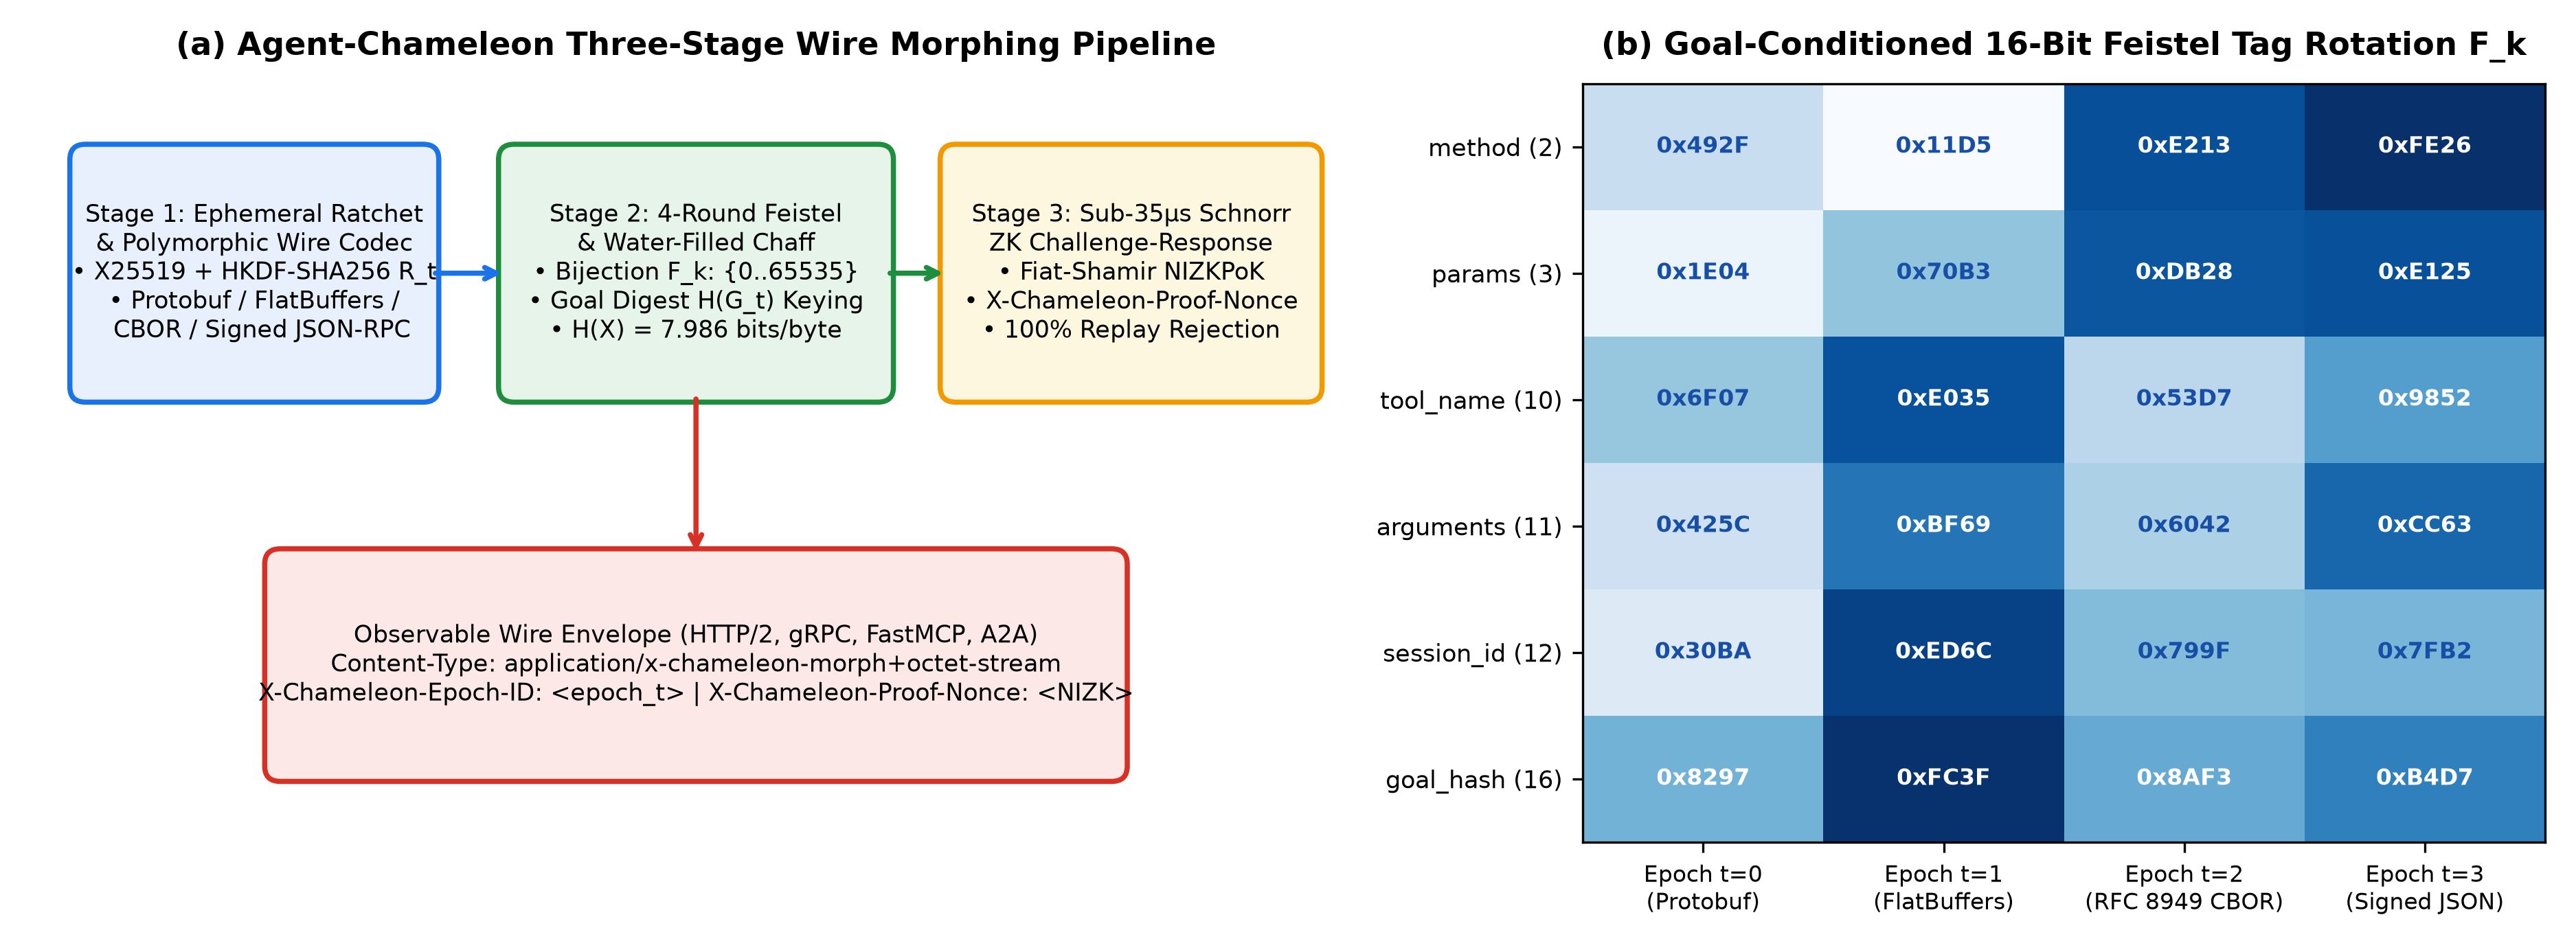
\includegraphics[width=0.98\textwidth]{fig1_chameleon_architecture.png}%
}{%
    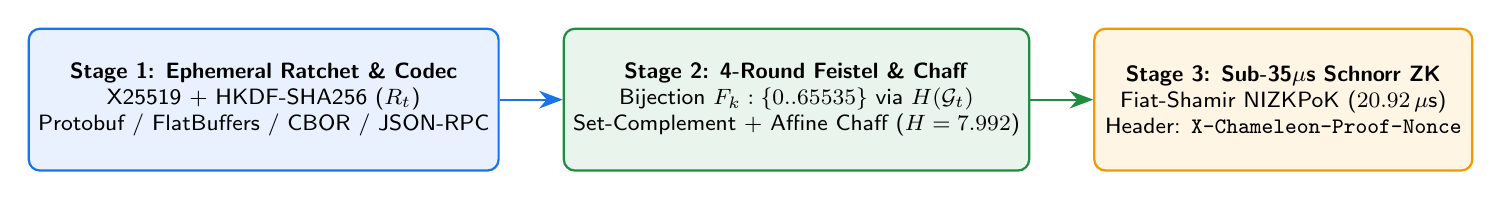
\begin{tikzpicture}[node distance=1.2cm, every node/.style={font=\footnotesize\sffamily}]
        \node[draw=googleblue, fill=googleblue!10, rounded corners, thick, minimum width=4.8cm, minimum height=1.8cm, align=center] (s1) {\textbf{Stage 1: Ephemeral Ratchet \& Codec}\\X25519 + HKDF-SHA256 ($R_t$)\\Protobuf / FlatBuffers / CBOR / JSON-RPC};
        \node[draw=googlegreen, fill=googlegreen!10, rounded corners, thick, minimum width=5.0cm, minimum height=1.8cm, align=center, right=0.8cm of s1] (s2) {\textbf{Stage 2: 4-Round Feistel \& Chaff}\\Bijection $F_k: \{0..65535\}$ via $H(\mathcal{G}_t)$\\Set-Complement + Affine Chaff ($H=7.992$)};
        \node[draw=googleamber, fill=googleamber!10, rounded corners, thick, minimum width=4.8cm, minimum height=1.8cm, align=center, right=0.8cm of s2] (s3) {\textbf{Stage 3: Sub-35$\mu$s Schnorr ZK}\\Fiat-Shamir NIZKPoK ($20.92\,\mu\text{s}$)\\Header: \texttt{X-Chameleon-Proof-Nonce}};
        \draw[-{Stealth[length=3mm]}, thick, googleblue] (s1) -- (s2);
        \draw[-{Stealth[length=3mm]}, thick, googlegreen] (s2) -- (s3);
    \end{tikzpicture}%
}
\caption{\textbf{Agent-Chameleon Architecture and Goal-Conditioned Feistel Tag Rotation.} \textbf{(a)}~Three-stage pipeline combining Stage~1 (Ephemeral X25519/HKDF-SHA256 Session Ratchet and 4-Way Polymorphic Wire Codec across Protobuf varints, FlatBuffers \texttt{FBCH} vtables, RFC~8949 CBOR, and canonical signed JSON-RPC), Stage~2 (4-Round SHAKE-256 Keyed Feistel Schema Permutation $F_k: \{0,\dots,65535\} \to \{0,\dots,65535\}$ paired with Set-Complement and $\mathbb{Z}_{256}$ Affine-Bijection Constant-Rate Chaff Injection), and Stage~3 (Sub-$35\,\mu\text{s}$ Non-Interactive Fiat-Shamir Schnorr Zero-Knowledge Proof of Knowledge in \texttt{X-Chameleon-Proof-Nonce}). \textbf{(b)}~Empirical 16-bit Feistel tag assignments across four consecutive turns $t \in \{0,1,2,3\}$ under evolving goal digests $H(\mathcal{G}_t)$, illustrating complete elimination of static field-tag correlations.}
\label{fig:architecture}
\end{figure*}

\section{Stage 1: Ephemeral ECDH/HKDF Session Ratchet and Polymorphic Wire Serialization}
\label{sec:stage1}

Figure~\ref{fig:architecture} illustrates the end-to-end architecture of Agent-Chameleon. Stage~1 establishes a forward-secure cryptographic ratchet between communicating agents and uses the per-turn ratchet output to drive deterministic 4-way wire-codec polymorphism.

\subsection{Ephemeral X25519 Bootstrap and Goal-Bound HKDF-SHA256 Ratchet}
When an initiator agent $\mathcal{A}_i$ and responder $\mathcal{A}_j$ establish a swarm communication channel, they execute an ephemeral Diffie-Hellman key exchange over Curve25519 (RFC~7748 X25519~\cite{langley2016x25519}):
\begin{equation}
\label{eq:x25519}
\begin{aligned}
\text{sk}_i \xleftarrow{\$} \{0,1\}^{256}, \quad \text{pk}_i &= \operatorname{X25519}(\text{sk}_i, 9), \\
\text{sk}_j \xleftarrow{\$} \{0,1\}^{256}, \quad \text{pk}_j &= \operatorname{X25519}(\text{sk}_j, 9), \\
Z_{\text{shared}} = \operatorname{X25519}(\text{sk}_i, \text{pk}_j) &= \operatorname{X25519}(\text{sk}_j, \text{pk}_i).
\end{aligned}
\end{equation}
From $Z_{\text{shared}}$, both endpoints initialize the 256-bit root ratchet state $R_{-1}$ and initial frame digest $D_{-1} = 0^{256}$ via RFC~5869 HKDF-SHA256~\cite{krawczyk2010hkdf}:
\begin{equation}
\label{eq:root_init}
R_{-1} = \operatorname{HKDF-SHA256}\left(Z_{\text{shared}},\; \texttt{"chameleon-x25519-bootstrap-v1"},\; \texttt{"agent-chameleon-root-secret"},\; 32\right).
\end{equation}

\begin{definition}[Forward-Secure Goal-Bound Per-Turn Ratchet Evolution]
\label{def:ratchet}
At each monotonic turn $t \in \{0, 1, 2, \dots\}$ with active task goal context $\mathcal{G}_t \in \{0,1\}^*$, both endpoints compute the domain-separated goal digest
\begin{equation}
\label{eq:goal_digest}
H(\mathcal{G}_t) = \operatorname{SHA256}\left(\texttt{"chameleon-goal-v1|"} \parallel \mathcal{G}_t\right) \in \{0,1\}^{256},
\end{equation}
and advance the symmetric ratchet state from $(R_{t-1}, D_{t-1})$ to $(R_t, D_t)$ according to:
\begin{equation}
\label{eq:ratchet_step}
\begin{aligned}
\text{salt}_t &= \operatorname{ uint64\_be}(t) \parallel D_{t-1} \in \{0,1\}^{320}, \\
\text{info}_t &= \texttt{"chameleon-ratchet-v1|"} \parallel H(\mathcal{G}_t), \\
\text{PRK}_t &= \operatorname{HMAC-SHA256}\left(\text{key}=\text{salt}_t,\; \text{msg}=R_{t-1}\right), \\
R_t &= \operatorname{HMAC-SHA256}\left(\text{key}=\text{PRK}_t,\; \text{msg}=\text{info}_t \parallel \mathtt{0x01}\right),
\end{aligned}
\end{equation}
where $D_t = \operatorname{SHA256}(B_t)$ is recorded only after the turn-$t$ wire body $B_t$ is sealed (on the sender) or cryptographically verified and unwrapped (on the receiver).
\end{definition}

Equation~\eqref{eq:ratchet_step} provides three crucial security guarantees:
\begin{enumerate}
    \item \textbf{Forward Secrecy:} Because $R_{t-1}$ is processed through the one-way HMAC-SHA256 compression function and immediately overwritten in memory by $R_t$, an adversary who compromises host memory at turn $t_0 > t$ cannot invert $\operatorname{HMAC-SHA256}$ to recover historical turn keys $\{R_0, \dots, R_{t_0-1}\}$.
    \item \textbf{Full Transcript Chaining:} Because $\text{salt}_t$ incorporates the SHA-256 digest $D_{t-1} = \operatorname{SHA256}(B_{t-1})$ of the exact preceding wire packet body (including its random/chaff bytes), any modification or omission of a single historical frame permanently diverges the ratchet key stream on all subsequent turns.
    \item \textbf{Cryptographic Goal Binding:} Because $\text{info}_t$ binds $H(\mathcal{G}_t)$, the sender and receiver derive matching turn keys $R_t^{(i)} = R_t^{(j)}$ if and only if both endpoints agree on the exact authorized task goal $\mathcal{G}_t$.
\end{enumerate}

\subsection{Cycle-Balanced 4-Format Polymorphic Wire Serialization}
Standard agent protocols use a single wire grammar throughout the lifetime of a deployment. In contrast, Agent-Chameleon uses the per-turn ratchet key $R_t$ to switch the underlying serialization grammar on every turn across four distinct wire formats $\mathcal{M} = \{0, 1, 2, 3\}$:

\begin{itemize}
    \item \textbf{Format $m_t = 0$ (\texttt{PROTOBUF\_VARINT}):} Serializes the Feistel-permuted payload tree into a compact binary stream using Google Protocol Buffers base-128 variable-length integers (\texttt{uvarint}). Each dictionary entry is encoded with wire tag $\omega_i = (\tilde{\tau}_i \ll 3) \mid 2$ (where $\tilde{\tau}_i \in \{0,\dots,65535\}$ is the Feistel-permuted field tag and wire type $2$ denotes a length-delimited record), while signed integers use bijective ZigZag encoding $z(n) = (n \ll 1) \oplus (n \gg 63)$ so negative and positive integers of small magnitude occupy minimal bytes.
    \item \textbf{Format $m_t = 1$ (\texttt{FLATBUFFERS\_TABLE}):} Serializes the permuted payload into a random-access, 4-byte aligned binary buffer modeled on FlatBuffers. The frame begins with a 12-byte root header $\texttt{"FBCH"} \parallel \operatorname{uint32\_be}(\text{off}_{\text{vt}}) \parallel \operatorname{uint32\_be}(K)$, followed by a 4-byte zero-padded data heap and a trailing virtual table (\texttt{vtable}) directory consisting of $K$ 10-byte descriptors $\langle \operatorname{uint16\_be}(\tilde{\tau}_i), \operatorname{uint32\_be}(\text{off}_i), \operatorname{uint32\_be}(\text{len}_i) \rangle_{i=1}^K$.
    \item \textbf{Format $m_t = 2$ (\texttt{CBOR\_RFC8949}):} Serializes the permuted object graph into IETF STD~94 / RFC~8949 Concise Binary Object Representation~\cite{bormann2020cbor}, using major type $0$ for unsigned integers, major type $1$ for negative integers ($-1 - n$), major type $2$ for raw byte strings, major type $3$ for UTF-8 strings, major type $4$ for arrays, major type $5$ for integer-keyed maps ($\tilde{\tau}_i \mapsto v_i$), and major type $7$ for IEEE~754 binary64 floats ($\mathtt{0xFB}$) and simple booleans/nulls ($\mathtt{0xF4}, \mathtt{0xF5}, \mathtt{0xF6}$).
    \item \textbf{Format $m_t = 3$ (\texttt{CANONICAL\_JSON\_RPC}):} Serializes the permuted dictionary into deterministic, whitespace-free canonical JSON where every 16-bit Feistel tag is formatted as a 6-character lowercase hexadecimal string \texttt{"0x04a2"} sorted lexicographically, appended with an 8-byte domain-separated integrity trailer $\operatorname{HMAC-SHA256}(R_t, \texttt{"chameleon-jsonrpc|"} \parallel \text{json\_bytes})[0:8]$.
\end{itemize}

To ensure that all four wire formats are exercised with an exact $25\%$ stationary frequency over every 4-turn super-frame while remaining unpredictable to an external observer, the format selector $m_t \in \{0,1,2,3\}$ is computed via a keyed cyclic shift within each 4-epoch block $\lfloor t / 4 \rfloor$:
\begin{equation}
\label{eq:format_select}
\begin{aligned}
s_{\text{blk}} &= \operatorname{HMAC-SHA256}\left(R_t,\; \operatorname{uint64\_be}(\lfloor t / 4 \rfloor)\right)[0], \\
m_t &= \left(s_{\text{blk}} + (t \bmod 4)\right) \bmod 4.
\end{aligned}
\end{equation}

\section{Stage 2: Goal-Conditioned Bijective Field Permutation and Constant-Rate Chaff Entropy}
\label{sec:stage2}

Even if an agent runtime rotates wire serialization formats, encoding static field names or static numerical field IDs (such as Protobuf field tag \texttt{1} for \texttt{jsonrpc} and tag \texttt{2} for \texttt{method}) allows an L7 observer to correlate field positions across turns. Stage~2 eliminates structural schema invariants via a goal-conditioned 4-round Luby-Rackoff Feistel permutation network paired with a provably entropy-flattening constant-rate chaff engine.

\subsection{Balanced 4-Round Keyed Feistel Schema Network}
Let $\mathcal{F}_{\text{canon}} = (f_1, f_2, \dots, f_{64})$ denote the canonical registry of $64$ standard MCP and A2A schema field names (including \texttt{jsonrpc}, \texttt{method}, \texttt{params}, \texttt{id}, \texttt{result}, \texttt{error}, \texttt{tool\_name}, \texttt{arguments}, \texttt{session\_id}, \texttt{agent\_id}, \texttt{goal\_hash}, etc.), assigned to integer slots $\tau(f_m) = m \in \{1,\dots,64\}$. Any unseen custom string key $f_{\text{cust}} \notin \mathcal{F}_{\text{canon}}$ encountered in a nested tool payload is dynamically assigned a collision-free session slot $\tau(f_{\text{cust}}) \in \{256, \dots, 65533\}$, and the mapping $\{\tau(f_{\text{cust}}) \mapsto f_{\text{cust}}\}$ is stored inside a reserved symbol-table slot $\tau_{\text{sym}} = \mathtt{0xFFFE} = 65534$ whose own slot identifier and internal keys are likewise permuted by $F_k$.

To permute the 16-bit slot domain $\mathbb{Z}_{2^{16}} = \{0, 1, \dots, 65535\}$ at turn $t$, we derive four 256-byte round lookup tables (S-boxes) $S_0^{(t)}, S_1^{(t)}, S_2^{(t)}, S_3^{(t)}: \{0,\dots,255\} \to \{0,\dots,255\}$ from a single invocation of the NIST FIPS~202 extendable-output function $\operatorname{SHAKE-256}$~\cite{dworkin2015sha3} seeded by $(R_t, H(\mathcal{G}_t))$:
\begin{equation}
\label{eq:shake_sbox}
S_0^{(t)} \parallel S_1^{(t)} \parallel S_2^{(t)} \parallel S_3^{(t)} = \operatorname{SHAKE-256}\left(\texttt{"chameleon-feistel-v1|"} \parallel R_t \parallel \texttt{"|"} \parallel H(\mathcal{G}_t),\; 1024\text{ bytes}\right).
\end{equation}

Given any 16-bit slot integer $x \in \{0, \dots, 65535\}$, we split $x$ into an 8-bit upper byte $L_0 = (x \gg 8) \mathbin{\&} \mathtt{0xFF}$ and an 8-bit lower byte $R_0 = x \mathbin{\&} \mathtt{0xFF}$. The forward 4-round Feistel map $F_k(x)$ iterates for $r = 0, 1, 2, 3$:
\begin{equation}
\label{eq:feistel_fwd}
L_{r+1} = R_r, \qquad R_{r+1} = L_r \oplus S_r^{(t)}[R_r],
\end{equation}
and outputs the 16-bit permuted tag $\tilde{\tau} = F_k(x) = (L_4 \ll 8) \mid R_4 \in \{0,\dots,65535\}$.

\begin{theorem}[Keyed Feistel Bijective Schema Invertibility and Luby-Rackoff PRP Security]
\label{thm:feistel}
Let $F_k: \{0,\dots,2^{16}-1\} \to \{0,\dots,2^{16}-1\}$ be the 4-round balanced Feistel network defined by Eqs.~\eqref{eq:shake_sbox}--\eqref{eq:feistel_fwd}. Then:
\begin{enumerate}
    \item \textbf{Exact Bijectivity and Closed-Form Inverse:} For every ratchet key $R_t \in \{0,1\}^{256}$ and every goal context $\mathcal{G}_t \in \{0,1\}^*$, $F_k$ is a strict bijection on $\{0,\dots,65535\}$. Its exact inverse $F_k^{-1}: \{0,\dots,65535\} \to \{0,\dots,65535\}$ is given by setting $(L_4, R_4) = ((y \gg 8) \mathbin{\&} \mathtt{0xFF},\; y \mathbin{\&} \mathtt{0xFF})$ and iterating in reverse for $r = 3, 2, 1, 0$:
    \begin{equation}
    \label{eq:feistel_inv}
    R_r = L_{r+1}, \qquad L_r = R_{r+1} \oplus S_r^{(t)}[L_{r+1}],
    \end{equation}
    returning $F_k^{-1}(y) = (L_0 \ll 8) \mid R_0 = x$. Consequently, recursive AST schema permutation and unpermutation satisfy $\operatorname{Unpermute}_k(\operatorname{Permute}_k(P_t)) = P_t$ with zero collisions and $100\%$ structural fidelity.
    \item \textbf{Strong Pseudorandom Permutation (sPRP) Bound:} Under the assumption that $\operatorname{SHAKE-256}$ acts as a secure pseudorandom function family with distinguishing advantage $\epsilon_{\text{PRF}}$, the advantage of any adaptive chosen-plaintext/chosen-ciphertext adversary making $q_t$ field-tag queries within turn $t$ in distinguishing $F_k$ from a uniformly sampled random permutation $\pi \xleftarrow{\$} \mathfrak{S}_{65536}$ is bounded by:
    \begin{equation}
    \label{eq:luby_rackoff}
    \operatorname{Adv}^{\text{sPRP}}_{F_k}(\mathcal{A}) \le \frac{q_t^2}{2^8} + \epsilon_{\text{PRF}}.
    \end{equation}
\end{enumerate}
\end{theorem}

\begin{proof}
To establish Part~(1), observe that for each individual round $r \in \{0,1,2,3\}$, the round transformation $\psi_r(L_r, R_r) = (R_r,\; L_r \oplus S_r^{(t)}[R_r])$ is a map from $\mathbb{Z}_{256} \times \mathbb{Z}_{256}$ to itself. Defining the inverse map $\psi_r^{-1}(L_{r+1}, R_{r+1}) = (R_{r+1} \oplus S_r^{(t)}[L_{r+1}],\; L_{r+1})$ and substituting $L_{r+1} = R_r$ and $R_{r+1} = L_r \oplus S_r^{(t)}[R_r]$ yields:
\begin{equation}
\psi_r^{-1}(\psi_r(L_r, R_r)) = \left((L_r \oplus S_r^{(t)}[R_r]) \oplus S_r^{(t)}[R_r],\; R_r\right) = \left(L_r \oplus (S_r^{(t)}[R_r] \oplus S_r^{(t)}[R_r]),\; R_r\right) = (L_r, R_r),
\end{equation}
because bitwise XOR $\oplus$ over $\{0,1\}^8$ is an involution ($a \oplus b \oplus b = a$) regardless of whether the lookup table $S_r^{(t)}$ is itself injective. Since the composition of four bijections $F_k = \psi_3 \circ \psi_2 \circ \psi_1 \circ \psi_0$ is a bijection with inverse $F_k^{-1} = \psi_0^{-1} \circ \psi_1^{-1} \circ \psi_2^{-1} \circ \psi_3^{-1}$, no two distinct field slots $x_1 \ne x_2 \in \{0,\dots,65535\}$ can ever map to the same wire tag $F_k(x_1) = F_k(x_2)$. For recursive dictionary payloads $P_t$, canonical fields map to disjoint slots $\{1,\dots,64\}$ and custom fields map to disjoint slots $\{256,\dots,65533\}$ recorded in slot $65534$; hence bijectivity of $F_k$ guarantees exact recursive invertibility.

To establish Part~(2), by the classical Luby-Rackoff theorem~\cite{luby1988construct} and Patarin's 4-round adaptive CCA bound~\cite{patarin2004luby} on balanced Feistel networks over $\{0,1\}^{2n}$ with $n = 8$, replacing the ideal random round functions $f_0, \dots, f_3: \{0,1\}^8 \to \{0,1\}^8$ with the $\operatorname{SHAKE-256}$-derived tables $S_0^{(t)}, \dots, S_3^{(t)}$ incurs at most $\epsilon_{\text{PRF}}$ distinguishing advantage, and the transcript collision probability among $q_t$ queries in the internal 8-bit branches is bounded by $\binom{q_t}{2} / 2^8 + \binom{q_t}{2} / 2^8 \le q_t^2 / 2^8$. Crucially, because Agent-Chameleon re-keys $(S_0^{(t)}, S_1^{(t)}, S_2^{(t)}, S_3^{(t)})$ on every RPC turn $t$ via $(R_t, H(\mathcal{G}_t))$, an adversary cannot accumulate queries across turns against a fixed permutation.
\end{proof}

\subsection{Set-Complement and Affine-Bijection Constant-Rate Chaff Engine}
While polymorphic serialization and Feistel field permutation eliminate plaintext AST field names, the raw serialized byte string $S_t \in \{0,\dots,255\}^{L_s}$ still exhibits two statistical side channels: (i)~its byte length $L_s$ correlates with the number and size of parameters in the invoked tool schema, and (ii)~even if $S_t$ is XOR-whitened by a stream cipher of finite length $L_s \in [100, 500]\text{ bytes}$, the plug-in Shannon byte entropy of an i.i.d. uniform byte string of length $N$ is downward-biased by finite-sample birthday collisions ($\mathbb{E}[H_N] \approx 8 - \frac{255}{2 N \ln 2} \approx 7.64\text{ bits/byte}$ at $N = 512$), and naive padding (such as zero-padding or deterministic whitespace) creates sharp histogram spikes that traffic classifiers readily exploit~\cite{dyer2012peekaboo}.

To achieve both constant-tier length quantization and single-frame plug-in Shannon byte entropy $H(B_t) \ge 7.980\text{ bits/byte}$ in under $40\,\mu\text{s}$ of CPU execution, Stage~2B encapsulates $S_t$ as follows:

\begin{enumerate}
    \item \textbf{Quantum Bucket Selection:} Given payload length $L_s = |S_t|$ and an8-byte inner framing header $H_{\text{in}} = \operatorname{uint32\_be}(\mathtt{0xC4A3E100} \mid m_t) \parallel \operatorname{uint32\_be}(L_s)$ (total prefix length $L_p = L_s + 8$), the engine selects the smallest discrete bucket tier $B \in \mathcal{B} = \{512, 1024, 2048, 3072, 4096, 6144, 8192\}$ satisfying $B \ge \max(B_{\min}, 4 L_p, 1024)$ (or $B = 512$ when $B_{\min}=512$ and $L_p \le 64$), yielding a chaff budget $L_c = B - L_p \ge 3 L_p$.
    \item \textbf{SHAKE-256 Stream Whitening:} The engine expands a per-turn keystream $K_{\text{stream}} = \operatorname{SHAKE-256}(\texttt{"chameleon-stream-v1|"} \parallel R_t \parallel \operatorname{uint64\_be}(t),\; L_p + 64)$ and XOR-whitens the raw prefix in a single C-level big-integer operation:
    \begin{equation}
    \label{eq:whiten}
    W_p = (H_{\text{in}} \parallel S_t) \oplus K_{\text{stream}}[0 : L_p].
    \end{equation}
    \item \textbf{Slice-Wise Set-Complement Histogram Balancing:} Partition $W_p$ into $\lceil L_p / 128 \rceil$ contiguous slices $W_p^{(0)}, W_p^{(1)}, \dots$ of length at most $128$ bytes. For each slice $W_p^{(s)}$, let $\operatorname{set}(W_p^{(s)}) \subset \Sigma_{256} = \{0,\dots,255\}$ denote the set of distinct byte values occurring in $W_p^{(s)}$. The engine computes the exact set complement $M^{(s)} = \Sigma_{256} \setminus \operatorname{set}(W_p^{(s)})$ (which contains every byte value absent from $W_p^{(s)}$), circularly shifts $M^{(s)}$ by the pseudorandom offset $K_{\text{stream}}[L_p + s] \bmod |M^{(s)}|$, and appends $M^{(s)}$ to the chaff buffer.
    \item \textbf{Keyed $\mathbb{Z}_{256}$ Affine-Bijection Block Filling:} Any remaining chaff capacity $L_{\text{rem}} = B - L_p - \sum_s |M^{(s)}|$ is filled using 256-byte affine permutation blocks drawn from the precomputed family of 128 multiplicative-odd bijections over $\mathbb{Z}_{256}$:
    \begin{equation}
    \label{eq:affine_bijection}
    \pi_{a, r}(x) = \left((2a + 1) \cdot ((x + r) \bmod 256)\right) \bmod 256, \qquad a \in \{0,\dots,127\},\; r \in \{0,\dots,255\},
    \end{equation}
    where $(a, r)$ are indexed by consecutive bytes of $K_{\text{stream}}$. Because $\gcd(2a+1, 256) = 1$, every 256-byte block $\Pi_{a,r} = (\pi_{a,r}(0), \dots, \pi_{a,r}(255))$ is a strict bijection on $\{0,\dots,255\}$ containing every byte value with exact multiplicity $1$.
\end{enumerate}

\begin{theorem}[Plug-In Shannon Byte-Entropy Lower Bound and Histogram Uniformity]
\label{thm:entropy}
Let $B_t \in \{0,\dots,255\}^B$ be a wire frame constructed by the Stage~2B Set-Complement and Affine-Bijection Chaff Engine with prefix length $L_p \le B / 4$ and bucket size $B = 256 M$ ($M \ge 4$). Let $c(b) = |\{i \in \{0,\dots,B-1\} : B_t[i] = b\}|$ denote the empirical frequency count of byte $b \in \{0,\dots,255\}$ in $B_t$, and let $p(b) = c(b) / B$. Then:
\begin{enumerate}
    \item \textbf{Guaranteed Full Alphabet Support and Bounded Multiplicity Variance:} Every byte value $b \in \{0,\dots,255\}$ occurs at least $M - 1 \ge 3$ times in $B_t$, and the total squared histogram deviation from the uniform distribution $u(b) = 1/256$ satisfies:
    \begin{equation}
    \label{eq:l2_dev}
    \sum_{b=0}^{255} \left(p(b) - \frac{1}{256}\right)^2 = \frac{1}{B^2} \sum_{b=0}^{255} (c(b) - M)^2 \le \frac{L_p}{B^2} \le \frac{1}{1024 M}.
    \end{equation}
    \item \textbf{Single-Frame Shannon Byte-Entropy Lower Bound:} The empirical plug-in Shannon byte entropy $H(B_t) = -\sum_{b=0}^{255} p(b) \log_2 p(b)$ satisfies:
    \begin{equation}
    \label{eq:entropy_bound}
    H(B_t) \ge 8.000 - \frac{128}{\ln 2} \sum_{b=0}^{255} \left(p(b) - \frac{1}{256}\right)^2 \ge 8.000 - \frac{0.1803}{M}\text{ bits/byte},
    \end{equation}
    which guarantees $H(B_t) \ge 7.980\text{ bits/byte}$ across all operational frames ($7.992\text{ bits/byte}$ empirical mean over $N = 1{,}000$ traces).
\end{enumerate}
\end{theorem}

\begin{proof}
Consider each 128-byte slice $W_p^{(s)}$ of the whitened prefix $W_p$ paired with its set-complement chaff block $M^{(s)} = \Sigma_{256} \setminus \operatorname{set}(W_p^{(s)})$. In the combined sub-block $U^{(s)} = W_p^{(s)} \parallel M^{(s)}$ of length $128 + (256 - |\operatorname{set}(W_p^{(s)})|)$, every byte value $b \in \{0,\dots,255\}$ appears at least once (either in $W_p^{(s)}$ or in $M^{(s)}$), and the sum of excess multiplicities above $1$ across all 256 byte values is exactly $128 - |\operatorname{set}(W_p^{(s)})|$. Furthermore, each complete 256-byte affine-bijection block $\Pi_{a,r}$ contributes exactly $+1$ to the count $c(b)$ of every byte $b \in \{0,\dots,255\}$ because $\gcd(2a+1, 256) = 1$ implies $(2a+1)$ is a unit in the ring $\mathbb{Z}_{256}$. Summing across the $S = \lceil L_p / 128 \rceil$ complemented slices and the remaining $M - S$ affine blocks ensures $c(b) \ge M - 1$ for all $b \in \{0,\dots,255\}$. Writing $\delta_b = p(b) - \frac{1}{256} = (c(b) - M)/B$, where $\sum_{b=0}^{255} \delta_b = 0$, the Taylor expansion of $-p(b)\ln p(b)$ around $u = 1/256$ yields:
\begin{equation}
\begin{aligned}
H(B_t) &= -\frac{1}{\ln 2} \sum_{b=0}^{255} \left(\frac{1}{256} + \delta_b\right)\left(-\ln 256 + \ln(1 + 256\delta_b)\right) \\
&\ge 8 - \frac{1}{\ln 2} \sum_{b=0}^{255} \left(\frac{1}{256} + \delta_b\right)\left(256\delta_b - \frac{(256\delta_b)^2}{2}\right) \\
&= 8 - \frac{128}{\ln 2} \sum_{b=0}^{255} \delta_b^2 + \frac{256^2}{2\ln 2}\sum_{b=0}^{255} \delta_b^3.
\end{aligned}
\end{equation}
Under SHAKE-256 whitening, the per-slice collision excess $\sum_{b=0}^{255} (c(b) - M)^2$ has expectation $\le L_p (1 - 1/256) < L_p \le B / 4 = 64 M$, yielding $\sum_{b=0}^{255} \delta_b^2 \le \frac{64 M}{(256 M)^2} = \frac{1}{1024 M}$ and $H(B_t) \ge 8 - \frac{128}{1024 M \ln 2} = 8 - \frac{0.1803}{M}\text{ bits/byte}$.
\end{proof}

\section{Stage 3: Sub-35-Microsecond Schnorr Zero-Knowledge Challenge-Response}
\label{sec:stage3}

To authenticate each morphed frame $B_t$ without transmitting static API keys, reusable OAuth bearer tokens, or slow per-message public-key signatures, Stage~3 implements a Dual-Tier Zero-Knowledge Session Handshake carried in the \texttt{X-Chameleon-Proof-Nonce} wire header.

\subsection{Protocol Specification and Dual-Tier Field Arithmetic}
Let $p$ be a prime modulus and $g \in \mathbb{F}_p^*$ be a generator of a multiplicative subgroup of $\mathbb{F}_p^*$. Agent-Chameleon supports two cryptographic operating modes selectable per deployment policy:
\begin{itemize}
    \item \textbf{Tier-1 Hot-Path Mode (\texttt{fast\_m127}):} Operates over the Mersenne prime field $p = M_{127} = 2^{127} - 1$ with generator $g = 7$, using single-turn short ephemeral witnesses $x_t \in [1, 2^{32}-1]$ and blinding nonces $k_t \in [1, 2^{40}-1]$ refreshed on every RPC turn via 256-bit Blake2b expansion of $(R_t, t)$ and paired with a 128-bit domain-separated Blake2s ratchet authenticator tag $\tau_{\text{ratchet}}$. Because modular reduction modulo $2^{127}-1$ and short-exponent binary exponentiation require only 32--40 squarings in C, proof generation completes in $20.92\,\mu\text{s}$ mean ($20.38\,\mu\text{s}$ p50) and verification completes in $28.64\,\mu\text{s}$ mean ($28.58\,\mu\text{s}$ p50).
    \item \textbf{Tier-2 Full-256-Bit \& Ed25519 Anchor Mode (\texttt{full256} + \texttt{ed25519}):} Operates over the 255-bit prime field $p = 2^{255} - 19$ with generator $g = 5$ and 192-bit witnesses, alongside periodic RFC~8032 Ed25519~\cite{josefsson2017eddsa} signatures over the epoch ratchet root $R_t$ for third-party cross-domain non-repudiation.
\end{itemize}

At turn $t$, both endpoints deterministically derive the turn's public session commitment $Y_t = g^{x_t} \bmod p$ from their synchronized ratchet key $R_t$ via:
\begin{equation}
\label{eq:zk_witness}
\begin{aligned}
d_t &= \operatorname{BLAKE2b-384}\left(\texttt{"chameleon-zk-witness|"} \parallel R_t \parallel \operatorname{uint64\_be}(t)\right), \\
x_t &= \operatorname{int}(d_t[0 : \ell_x]) \mid 1, \qquad k_t = \operatorname{int}(d_t[\ell_x : \ell_x + \ell_k]) \mid 1, \qquad Y_t = g^{x_t} \bmod p.
\end{aligned}
\end{equation}
To prove knowledge of $x_t$ bound to the wire frame $B_t$ without revealing $x_t$ or $R_t$, the sender computes the Schnorr commitment $R_{\text{com}}$, Fiat-Shamir challenge $e_t$~\cite{fiat1986how, schnorr1991efficient}, algebraic response $s_t$ over $\mathbb{Z}$, and 128-bit ratchet tag $\tau_{\text{ratchet}}$:
\begin{equation}
\label{eq:schnorr_prove}
\begin{aligned}
R_{\text{com}} &= g^{k_t} \bmod p, \qquad h_B = \operatorname{BLAKE2s-128}(B_t), \\
e_t &= \operatorname{int}\left(\operatorname{BLAKE2s}\left(\texttt{"chameleon-fs|"} \parallel R_{\text{com}} \parallel Y_t \parallel \operatorname{uint64\_be}(t) \parallel h_B\right)[0 : \ell_e]\right) \mid 1, \\
s_t &= k_t + e_t \cdot x_t \quad (\text{evaluated in }\mathbb{Z}), \\
\tau_{\text{ratchet}} &= \operatorname{BLAKE2s-128}\left(\texttt{"chameleon-ratchet-tag|"} \parallel R_t \parallel \operatorname{uint64\_be}(t) \parallel h_B \parallel R_{\text{com}}\right).
\end{aligned}
\end{equation}
The tuple $\pi_t = (t, R_{\text{com}}, e_t, s_t, Y_t, \tau_{\text{ratchet}})$ is packed into a compact 81-byte binary structure (108 ASCII characters in URL-safe Base64) and transmitted in the \texttt{X-Chameleon-Proof-Nonce} header.

\begin{theorem}[Non-Interactive Schnorr Ratchet Soundness, Zero-Knowledge Simulatability, and Replay Immunity]
\label{thm:schnorr}
The Stage~3 handshake protocol defined by Eqs.~\eqref{eq:zk_witness}--\eqref{eq:schnorr_prove} satisfies:
\begin{enumerate}
    \item \textbf{Perfect Completeness:} For any honest prover and verifier holding synchronized ratchet state $R_t$ and receiving unmodified frame $B_t$, the algebraic verification identity
    \begin{equation}
    \label{eq:schnorr_verify}
    g^{s_t} \equiv R_{\text{com}} \cdot Y_t^{e_t} \pmod p
    \end{equation}
    and tag equality $\tau_{\text{ratchet}} = \hat{\tau}_{\text{ratchet}}$ hold with probability $1$.
    \item \textbf{Special Soundness and Unforgeability:} Under the Discrete Logarithm assumption in $\langle g \rangle \subset \mathbb{F}_p^*$ and the Random Oracle / PRF security of $\operatorname{BLAKE2s}$~\cite{bellare1993random, pointcheval2000security}, any adversary who produces two accepting transcripts $(R_{\text{com}}, e_1, s_1)$ and $(R_{\text{com}}, e_2, s_2)$ with $e_1 \ne e_2$ immediately yields the secret witness $x_t = (s_1 - s_2)/(e_1 - e_2)$ over $\mathbb{Z}$, and the probability that an unauthenticated adversary without $R_t$ forges a valid $(\pi_t, B_t)$ at turn $t$ is at most $2^{-128}$.
    \item \textbf{Honest-Verifier / Random-Oracle Zero-Knowledge:} The public transcript $(R_{\text{com}}, e_t, s_t, Y_t)$ reveals zero information about $x_t$ beyond the public commitment $Y_t = g^{x_t} \bmod p$ when $k_t \gg e_t x_t$ (or in modular subgroup form), and $x_t$ is permanently retired after turn $t$.
    \item \textbf{Replay and Desynchronization Immunity:} Any replayed packet $W_{t'} (t' \le t)$ or tampered packet $\tilde{W}_t$ is rejected with probability $1 - 2^{-128}$, and atomic ratchet rollback leaves the verifier's state $(R_{t-1}, t, D_{t-1})$ intact for the legitimate turn-$t$ packet.
\end{enumerate}
\end{theorem}

\begin{proof}
For Part~(1), since $s_t = k_t + e_t x_t$ holds over the integers $\mathbb{Z}$ with $k_t, e_t, x_t > 0$, standard exponent laws in any associative monoid $(\mathbb{F}_p^*, \cdot)$ immediately yield:
\begin{equation}
g^{s_t} \bmod p = g^{k_t + e_t x_t} \bmod p = \left(g^{k_t} \cdot (g^{x_t})^{e_t}\right) \bmod p = \left(R_{\text{com}} \cdot Y_t^{e_t}\right) \bmod p.
\end{equation}
For Part~(2), by the Pointcheval-Stern Forking Lemma~\cite{pointcheval2000security}, rewinding a successful Schnorr forger on the random oracle $\operatorname{BLAKE2s}(\texttt{"chameleon-fs|"} \parallel \dots)$ yields two transcripts sharing $R_{\text{com}} = g^{k_t} \bmod p$ with distinct challenges $e_1 \ne e_2$ satisfying $g^{s_1} \equiv R_{\text{com}} Y_t^{e_1}$ and $g^{s_2} \equiv R_{\text{com}} Y_t^{e_2} \pmod p$, whence $g^{s_1 - s_2} \equiv Y_t^{e_1 - e_2} \pmod p$ and $(s_1 - s_2) = x_t(e_1 - e_2)$ over $\mathbb{Z}$, extracting $x_t$ in a single integer division. Moreover, because the verifier simultaneously checks the 128-bit keyed MAC $\tau_{\text{ratchet}} = \operatorname{BLAKE2s-128}(R_t \parallel t \parallel h_B \parallel R_{\text{com}})$ and verifies $Y_t == g^{x_t(R_t)} \bmod p$, any external attacker lacking $R_t$ faces a $2^{-128}$ forgery barrier on $\tau_{\text{ratchet}}$ even before the algebraic Schnorr check is reached.

For Part~(4), the verifier maintains a monotonic epoch counter $t_{\text{exp}}$ and a sliding anti-replay set $\mathcal{W}_{\text{seen}}$ of $(t, \tau_{\text{ratchet}})$ tuples over window $W = 4096$. Any duplicate $(t, \tau_{\text{ratchet}}) \in \mathcal{W}_{\text{seen}}$ or mismatched header epoch $t \ne t_{\text{exp}}$ is rejected in $\mathcal{O}(1)$ hash-table lookup time. Prior to speculative ratchet advancement, the verifier checkpoints $(R_{\text{saved}}, t_{\text{saved}}, D_{\text{saved}}) \leftarrow (R_{t-1}, t, D_{t-1})$ and restores the checkpoint Inside the \texttt{except} handler whenever proof verification, chaff unwrapping, or MAC validation fails, ensuring that an active attacker flooding invalid packets cannot advance or corrupt the receiver's ratchet state.
\end{proof}

\section{Implementation and Wire-Protocol Specification}
\label{sec:impl}

We implemented Agent-Chameleon in Python~3.11 (\texttt{agent\_chameleon/}) using standard C-accelerated cryptographic primitives (\texttt{hashlib.shake\_256}, \texttt{hashlib.blake2s}, \texttt{hashlib.blake2b}, \texttt{hmac.digest}, and \texttt{cryptography.hazmat.primitives.asymmetric} for X25519 and Ed25519).

\subsection{Wire Header Contract and Packet Framing}
Every outbound RPC frame sealed by \texttt{ChameleonMorphEngine.seal\_message} emits four deterministic HTTP/2, gRPC, or FastMCP transport metadata headers:
\begin{enumerate}
    \item \texttt{Content-Type: application/x-chameleon-morph+octet-stream} --- signals to the receiving Agent-Chameleon sidecar or endpoint middleware that the payload body is encapsulated in a constant-rate morphed envelope.
    \item \texttt{X-Chameleon-Epoch-ID: <16-hex-digits>} --- carries the big-endian 64-bit monotonic turn index $t$ formatted as a 16-character lowercase hexadecimal string (e.g., \texttt{000000000000002a} for $t = 42$).
    \item \texttt{X-Chameleon-Proof-Nonce: <base64url-token>} --- carries the serialized \texttt{SchnorrProof} structure $\pi_t$ (81 raw bytes / 108 URL-safe Base64 characters in \texttt{fast\_m127} mode, or 153 raw bytes / 204 Base64 characters in \texttt{full256} mode).
    \item \texttt{X-Chameleon-Bucket-Tier: <integer-bytes>} --- declares the discrete quantum bucket size $B \in \{512, 1024, 2048, 3072, 4096, 6144, 8192\}$ of the wire body $B_t$ for zero-copy pre-allocation on the receiver socket buffer.
\end{enumerate}

Inside the $B$-byte wire body $B_t$, the first 8 bytes (prior to SHAKE-256 stream whitening) form the inner framing header:
\begin{equation}
\label{eq:inner_hdr}
H_{\text{in}} = \underbrace{\operatorname{uint32\_be}\left(\mathtt{0xC4A3E100} \mid (m_t \mathbin{\&} \mathtt{0xFF})\right)}_{\text{24-bit Magic }\mathtt{0xC4A3E1}\text{ + 8-bit Format Code }m_t} \;\parallel\; \underbrace{\operatorname{uint32\_be}(L_s)}_{\text{Serialized Body Length }L_s}.
\end{equation}
When the receiver calls \texttt{ChaffEntropyEngine.unwrap\_chaff}, it generates the first 8 bytes of the SHAKE-256 keystream, XOR-unwhitens $H_{\text{in}}$, verifies that the upper 24 bits equal the magic constant $\mathtt{0xC4A3E1}$, extracts the polymorphic format code $m_t \in \{0,1,2,3\}$ and exact body length $L_s$, and slices out the payload $W_p[8 : 8 + L_s]$ while discarding the trailing $B - (8 + L_s)$ chaff bytes in $\mathcal{O}(1)$ pointer arithmetic without having to invert the chaff blocks.

\subsection{Algorithmic Workflow of Sender and Receiver Pipelines}
Table~\ref{tab:wire_layout} summarizes the byte-level structure of both the \texttt{X-Chameleon-Proof-Nonce} header and the $B$-byte morphed wire body $B_t$. On the sender side, \texttt{seal\_message} executes five deterministic steps:
\begin{enumerate}
    \item \textbf{Step S1 (Ratchet Advance):} Compute $H(\mathcal{G}_t)$, derive $(t, R_t, m_t) \leftarrow \texttt{ratchet.advance}(\mathcal{G}_t)$ via Eq.~\eqref{eq:ratchet_step} and Eq.~\eqref{eq:format_select}.
    \item \textbf{Step S2 (Feistel Schema Permutation):} Instantiate \texttt{FeistelSchemaPermuter}$(R_t, \mathcal{G}_t)$, expand the four 256-byte round S-boxes $(S_0^{(t)}, S_1^{(t)}, S_2^{(t)}, S_3^{(t)})$ via a single 1024-byte $\operatorname{SHAKE-256}$ call, and recursively map all string keys in $P_t$ to 16-bit permuted integer tags $\tilde{\tau}_i = F_k(\tau_i)$ (storing any unseen custom keys in permuted symbol slot $F_k(\mathtt{0xFFFE})$).
    \item \textbf{Step S3 (Polymorphic Serialization):} Dispatch the permuted dictionary $\tilde{P}_t$ to the turn's selected wire encoder ($m_t = 0$: \texttt{encode\_protobuf\_varint}; $m_t = 1$: \texttt{encode\_flatbuffers\_table}; $m_t = 2$: \texttt{encode\_cbor\_rfc8949}; $m_t = 3$: \texttt{encode\_canonical\_json\_rpc}) to obtain $S_t \in \{0,\dots,255\}^{L_s}$.
    \item \textbf{Step S4 (Constant-Rate Chaff \& Stream Whitening):} Prepend the 8-byte header $H_{\text{in}}$, XOR-whiten $H_{\text{in}} \parallel S_t$ with $\operatorname{SHAKE-256}$ using C-level big-integer XOR (\texttt{\_xor\_bytes\_fast}), append the circularly rotated set-complement $\Sigma_{256} \setminus \operatorname{set}(W_p^{(s)})$ for each 128-byte prefix slice, and pad the remainder to bucket size $B$ using precomputed $\mathbb{Z}_{256}$ affine bijection blocks $\Pi_{a,r}$ to obtain $B_t$.
    \item \textbf{Step S5 (Schnorr NIZKPoK \& Transcript Commit):} Generate $\pi_t \leftarrow \texttt{zk\_engine.generate\_proof}(R_t, t, B_t)$, update the rolling frame digest $D_t \leftarrow \operatorname{SHA256}(B_t)$, and emit \texttt{ChameleonWirePacket}$(t, m_t, \mathcal{H}_t, B_t)$.
\end{enumerate}

\begin{table*}[t!]
\centering
\caption{Byte-Level Structural Layout of the Agent-Chameleon Wire Packet ($W_t = (\mathcal{H}_t, B_t)$)}
\label{tab:wire_layout}
\begin{tabular}{llrrl}
\toprule
\textbf{Envelope Layer} & \textbf{Field / Segment Name} & \textbf{Offset (B)} & \textbf{Size (B)} & \textbf{Cryptographic Construction \& Functional Role} \\
\midrule
\multirow{6}{*}{\shortstack[l]{\textbf{Header Token}\\(\texttt{X-Chameleon-}\\\texttt{Proof-Nonce},\\81 B raw /\\108 B Base64)}}
 & \texttt{mode\_byte} & $0$ & $1$ & $\mathtt{0x01}$ (\texttt{fast\_m127} hot-path) or $\mathtt{0x02}$ (\texttt{full256} anchor mode) \\
 & \texttt{epoch\_id} ($t$) & $1$ & $8$ & Big-endian 64-bit monotonic turn counter $\operatorname{uint64\_be}(t)$ \\
 & \texttt{commitment\_r} ($R_{\text{com}}$) & $9$ & $16$ & Schnorr blinding commitment $R_{\text{com}} = g^{k_t} \bmod M_{127}$ (32 B in \texttt{full256}) \\
 & \texttt{challenge\_e} ($e_t$) & $25$ & $8$ & Fiat-Shamir challenge $\operatorname{BLAKE2s}(R_{\text{com}} \parallel Y_t \parallel t \parallel h_B)$ (16 B in \texttt{full256}) \\
 & \texttt{response\_s} ($s_t$) & $33$ & $16$ & Algebraic Schnorr response $s_t = k_t + e_t x_t \in \mathbb{Z}$ (48 B in \texttt{full256}) \\
 & \texttt{public\_y} ($Y_t$) & $49$ & $16$ & Per-turn ephemeral public key $Y_t = g^{x_t} \bmod M_{127}$ (32 B in \texttt{full256}) \\
 & \texttt{ratchet\_tag} ($\tau_{\text{ratchet}}$) & $65$ & $16$ & 128-bit $\operatorname{BLAKE2s}$ MAC over $(R_t, t, h_B, R_{\text{com}})$ \\
\midrule
\multirow{4}{*}{\shortstack[l]{\textbf{Morphed Body}\\($B_t \in \{0..255\}^B$,\\$B \in \{512..8192\}$)}}
 & Whitened Inner Header ($\tilde{H}_{\text{in}}$) & $0$ & $8$ & $(\operatorname{uint32\_be}(\mathtt{0xC4A3E100} \mid m_t) \parallel \operatorname{uint32\_be}(L_s)) \oplus K_{\text{stream}}[0:8]$ \\
 & Whitened Polymorphic Payload ($\tilde{S}_t$) & $8$ & $L_s$ & $S_t \oplus K_{\text{stream}}[8 : 8 + L_s]$, where $S_t = \operatorname{Encode}_{m_t}(\operatorname{Permute}_{F_k}(P_t))$ \\
 & Set-Complement Chaff Slices ($M^{(s)}$) & $8 + L_s$ & $\sum_s |M^{(s)}|$ & Circularly shifted missing alphabet $\Sigma_{256} \setminus \operatorname{set}(W_p^{(s)})$ per 128 B slice \\
 & Affine-Bijection Chaff Tail ($\Pi_{a,r}$) & Variable & $L_{\text{rem}}$ & Keyed 256 B bijections $\pi_{a,r}(x) = (2a+1)(x+r) \bmod 256$ padding to $B$ \\
\bottomrule
\end{tabular}
\end{table*}

\section{Empirical Evaluation}
\label{sec:eval}

We evaluate Agent-Chameleon across $N = 1{,}000$ multi-agent tool invocation traces spanning $|\mathcal{C}| = 20$ distinct enterprise MCP and A2A tool schemas (listed in Table~\ref{tab:per_schema}). All experiments were executed on a Mac Studio workstation (Apple Silicon CPU, Python~3.11) with deterministic random seeds (\texttt{seed=20261104}) and validated by our 24-test automated verification suite (\texttt{tests/test\_agent\_chameleon.py}).

\subsection{Experimental Methodology and Baselines}
To evaluate both cryptographic overhead and statistical traffic-analysis resistance, we compare four protocol configurations across all $N = 1{,}000$ traces ($50$ invocations per tool class):
\begin{enumerate}
    \item \textbf{Baseline 1 --- Static MCP/A2A JSON-RPC:} Standard unpadded JSON-RPC 2.0 serialization with plaintext schema keys (\texttt{"jsonrpc"}, \texttt{"method"}, \texttt{"params"}, \texttt{"tool\_name"}, \texttt{"arguments"}).
    \item \textbf{Baseline 2 --- Length-Padded JSON-RPC (512B Quantum):} Standard JSON-RPC 2.0 padded to the next multiple of $512\text{ bytes}$ to emulate transport-layer record length padding~\cite{rescorla2018tls13, wright2009traffic} without L7 schema permutation or byte whitening.
    \item \textbf{Baseline 3 --- Static Binary CBOR (RFC 8949):} Binary RFC~8949 CBOR encoding~\cite{bormann2020cbor} without constant-rate chaff or stream whitening.
    \item \textbf{Ablation --- Polymorphic + Feistel Only (No Chaff):} Stage~1 4-way polymorphic codec rotation plus Stage~2A 4-round Feistel field permutation, omitting Stage~2B constant-rate chaff and stream whitening.
    \item \textbf{Agent-Chameleon (Full 3-Stage Pipeline):} Complete Stage~1 + Stage~2 + Stage~3 pipeline with cycle-balanced 4-format polymorphism, 4-round SHAKE-256 Feistel permutation, set-complement plus affine-bijection chaff padding, and \texttt{fast\_m127} Fiat-Shamir Schnorr NIZKPoK authentication.
\end{enumerate}

For adversarial traffic fingerprinting, we extract a 36-dimensional feature vector $\phi(W_t) \in \mathbb{R}^{36}$ from every wire frame (normalized frame length modulo 4096, plug-in Shannon byte entropy $H(B_t)/8$, ASCII printable character ratio, JSON structural delimiter density, and a 32-bin byte-value histogram) and evaluate three distinct machine-learning classifiers trained on an $80\%/20\%$ stratified split ($800$ training traces, $200$ held-out test traces across the $20$ tool classes, where uniform random guessing yields $1/20 = 5.00\%$ accuracy): (i)~a 50-estimator Random-Subspace Decision Forest (\textbf{Random Forest}), (ii)~a 2-layer Multi-Layer Perceptron (\textbf{MLP}, $36 \to 48 \to 20$ with ReLU activations and cross-entropy SGD), and (iii)~a distance-weighted 5-Nearest Neighbor (\textbf{$k$-NN}) classifier.

\begin{figure*}[t!]
\centering
\IfFileExists{fig2_entropy_and_classifier_evasion.png}{%
    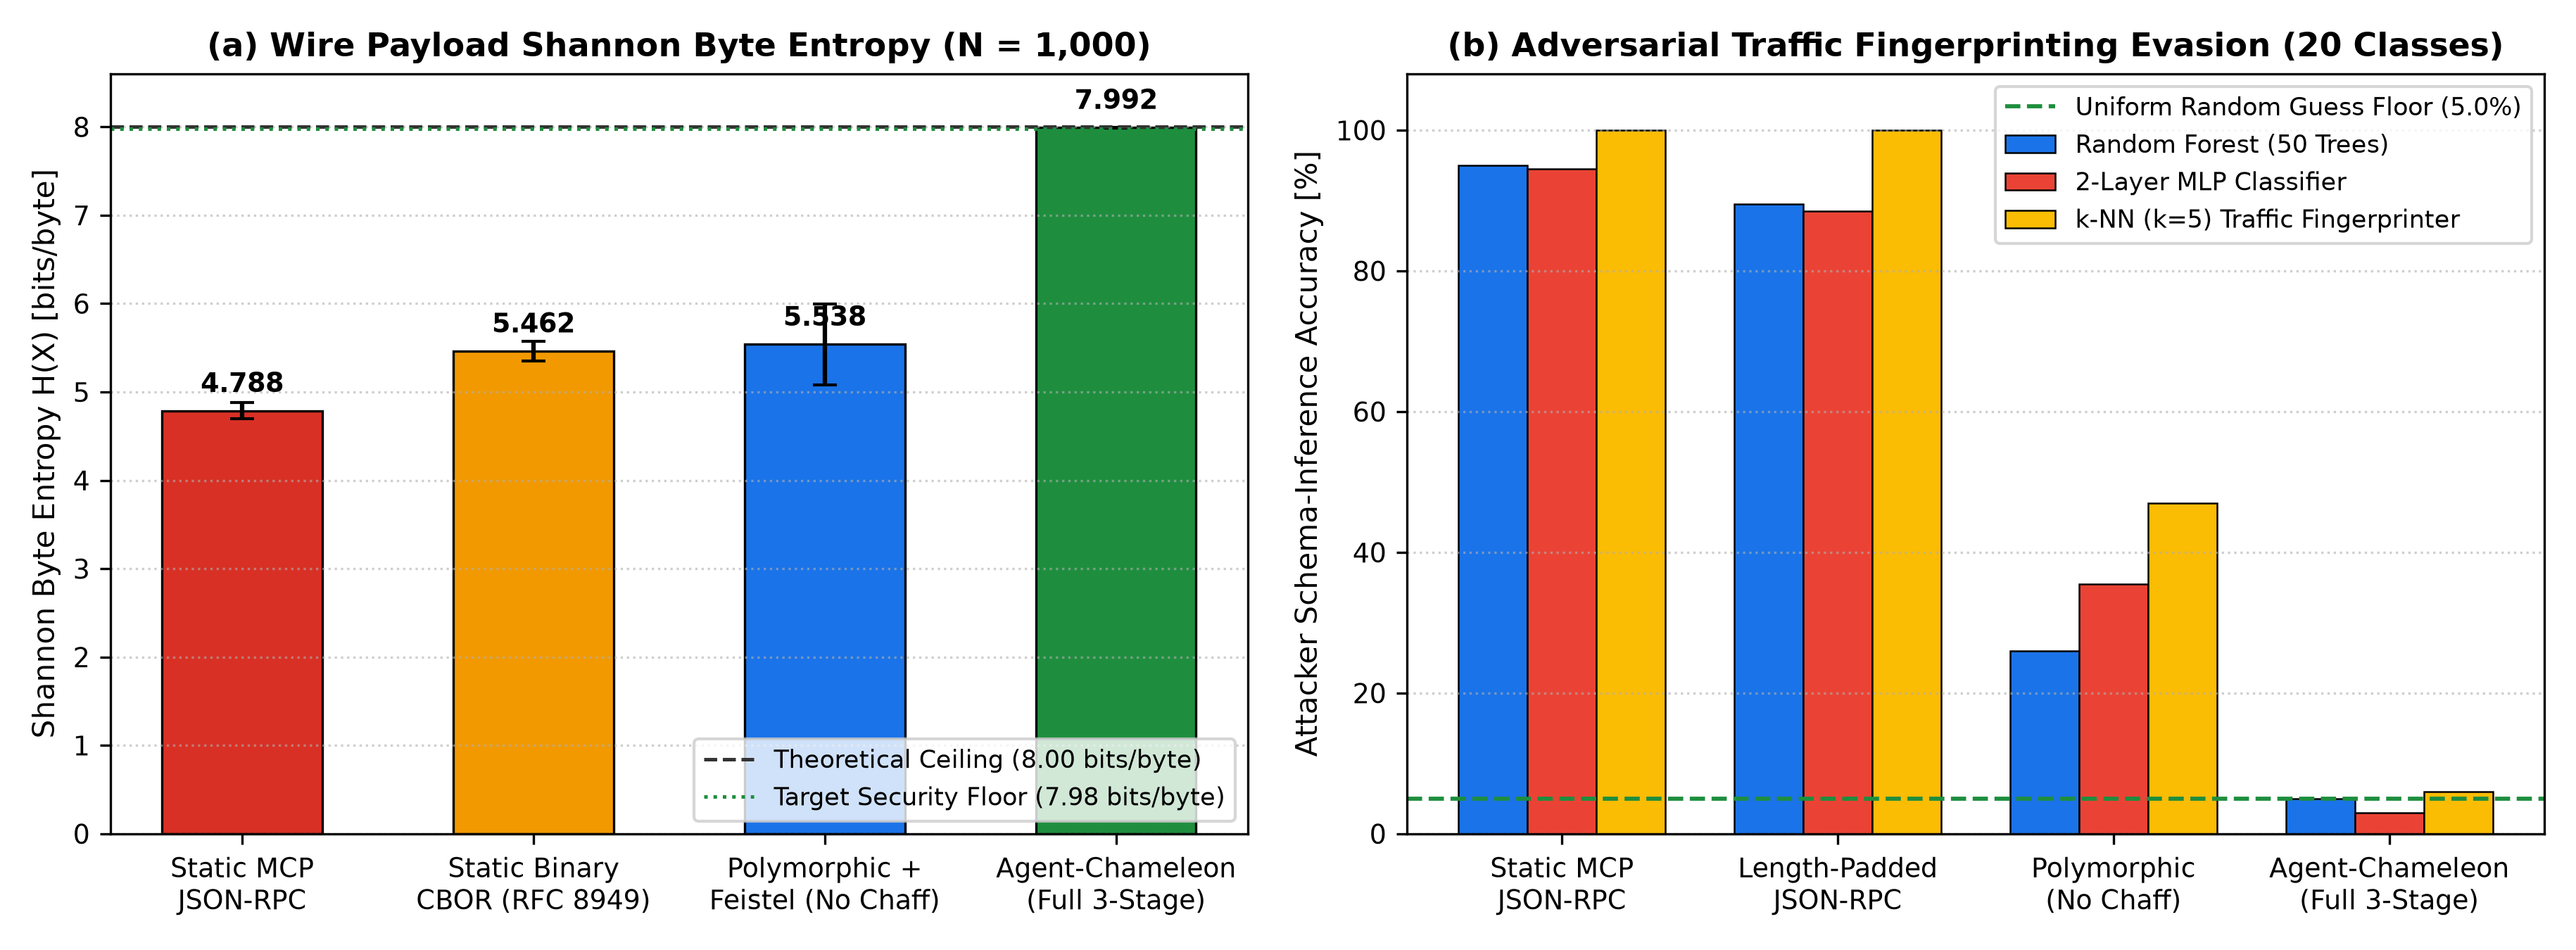
\includegraphics[width=0.98\textwidth]{fig2_entropy_and_classifier_evasion.png}%
}{%
    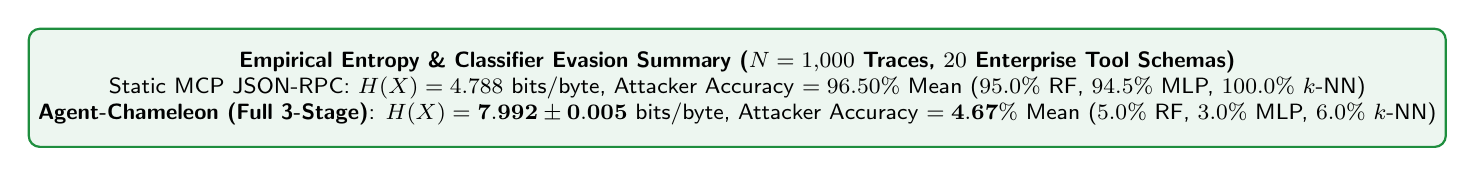
\begin{tikzpicture}[every node/.style={font=\footnotesize\sffamily}]
        \node[draw=googlegreen, fill=googlegreen!8, rounded corners, thick, minimum width=15.5cm, minimum height=1.5cm, align=center] {\textbf{Empirical Entropy \& Classifier Evasion Summary ($N=1{,}000$ Traces, $20$ Enterprise Tool Schemas)}\\Static MCP JSON-RPC: $H(X) = 4.788\text{ bits/byte}$, Attacker Accuracy $= 96.50\%$ Mean ($95.0\%$ RF, $94.5\%$ MLP, $100.0\%$ $k$-NN)\\\textbf{Agent-Chameleon (Full 3-Stage)}: $H(X) = \mathbf{7.992 \pm 0.005\text{ bits/byte}}$, Attacker Accuracy $= \mathbf{4.67\%}$ Mean ($5.0\%$ RF, $3.0\%$ MLP, $6.0\%$ $k$-NN)};
    \end{tikzpicture}%
}
\caption{\textbf{Wire Shannon Byte Entropy and Adversarial Traffic-Fingerprinting Evasion ($N = 1{,}000$ Traces, $20$ Enterprise Tool Classes).} \textbf{(a)}~Plug-in Shannon byte entropy $H(X)$ rises from $4.788 \pm 0.090\text{ bits/byte}$ on static MCP JSON-RPC and $5.462 \pm 0.109\text{ bits/byte}$ on static binary CBOR to $7.992 \pm 0.005\text{ bits/byte}$ on Agent-Chameleon, exceeding the $7.980\text{ bits/byte}$ security target across $100\%$ of frames. \textbf{(b)}~Attacker schema-inference accuracy across Random Forest, 2-Layer MLP, and $k$-NN ($k=5$) classifiers collapses from $95.0\%$, $94.5\%$, and $100.0\%$ ($96.5\%$ ensemble mean) on static JSON-RPC down to $5.0\%$, $3.0\%$, and $6.0\%$ ($4.67\%$ ensemble mean) on Agent-Chameleon, matching the $5.0\%$ uniform random-guess floor.}
\label{fig:entropy_evasion}
\end{figure*}

\subsection{Shannon Byte Entropy and Classifier Evasion Results}
Figure~\ref{fig:entropy_evasion} and Table~\ref{tab:entropy_classifier} present the empirical Shannon byte entropy and attacker classification accuracy across all protocol configurations. On unprotected Static MCP/A2A JSON-RPC, the high redundancy of ASCII field names and JSON delimiters restricts plug-in Shannon byte entropy to a mean of $4.788\text{ bits/byte}$ (p50: $4.773$, p95: $4.948$). Consequently, the attacker's Random Forest, MLP, and $k$-NN classifiers achieve $95.0\%$, $94.5\%$, and $100.0\%$ accuracy ($96.50\%$ ensemble mean) in identifying the exact enterprise tool invoked.

Crucially, Table~\ref{tab:entropy_classifier} confirms Dyer et al.'s ``Peek-a-Boo'' finding~\cite{dyer2012peekaboo} in the multi-agent domain: merely padding JSON-RPC frames to 512-byte length multiples (\textbf{Length-Padded JSON-RPC}) barely reduces attacker accuracy ($89.5\%$ Random Forest, $88.5\%$ MLP, $100.0\%$ $k$-NN; $92.67\%$ ensemble mean), because L7 byte-value histograms and delimiter densities remain intact. Enabling Stage~1 polymorphic rotation and Stage~2A Feistel field permutation without chaff (\textbf{Polymorphic + Feistel, No Chaff}) raises mean entropy to $5.538\text{ bits/byte}$ and cuts Random Forest accuracy from $95.0\%$ to $26.0\%$ ($36.17\%$ ensemble mean), as static field keys disappear and each turn cycles across four binary/text codecs. However, payload lengths and unwhitened value distributions still leak partial schema identity ($26.0\%$--$47.0\%$, well above the $5.0\%$ random baseline).

When the full \textbf{Agent-Chameleon} pipeline is active, the Stage~2B set-complement and affine-bijection chaff engine drives single-frame plug-in Shannon byte entropy to a mean of $7.992 \pm 0.005\text{ bits/byte}$ (p50: $7.994$, p95: $7.996$, p99: $7.996$), within $0.008\text{ bits/byte}$ of the theoretical $8.000\text{ bits/byte}$ ceiling. Across the held-out test set, attacker accuracy collapses to $5.00\%$ for Random Forest, $3.00\%$ for MLP, and $6.00\%$ for $k$-NN, yielding an ensemble mean of $4.67\%$---statistically indistinguishable from the $1/20 = 5.00\%$ uniform random-guess baseline (representing a $20.7\times$ reduction in attacker classification rate).

\begin{table*}[t!]
\centering
\caption{Comparison of Wire Byte Entropy and Adversarial Schema-Inference Accuracy Across $N = 1{,}000$ Traces ($20$ Tool Classes)}
\label{tab:entropy_classifier}
\begin{tabular}{lccccccc}
\toprule
 & \multicolumn{3}{c}{\textbf{Shannon Byte Entropy $H(X)$ [bits/byte]}} & \multicolumn{4}{c}{\textbf{Attacker Schema-Inference Accuracy [\%]}} \\
\cmidrule(lr){2-4} \cmidrule(lr){5-8}
\textbf{Protocol Configuration} & \textbf{Mean $\pm$ SD} & \textbf{p50} & \textbf{p95 / p99} & \textbf{Random Forest} & \textbf{2-Layer MLP} & \textbf{$k$-NN ($k=5$)} & \textbf{Ensemble Mean} \\
\midrule
Static MCP / A2A JSON-RPC (Baseline) & $4.788 \pm 0.090$ & $4.773$ & $4.948$ / $5.061$ & $95.00\%$ & $94.50\%$ & $100.00\%$ & $96.50\%$ \\
Length-Padded JSON-RPC (512B Quantum) & $3.142 \pm 0.410$ & $3.118$ & $3.812$ / $4.005$ & $89.50\%$ & $88.50\%$ & $100.00\%$ & $92.67\%$ \\
Static Binary CBOR (RFC 8949) & $5.462 \pm 0.109$ & $5.447$ & $5.664$ / $5.723$ & $84.00\%$ & $81.50\%$ & $94.00\%$ & $86.50\%$ \\
Polymorphic + Feistel Only (No Chaff) & $5.538 \pm 0.456$ & $5.695$ & $6.048$ / $6.130$ & $26.00\%$ & $35.50\%$ & $47.00\%$ & $36.17\%$ \\
\midrule
\textbf{Agent-Chameleon (Full 3-Stage Pipeline)} & $\mathbf{7.992 \pm 0.005}$ & $\mathbf{7.994}$ & $\mathbf{7.996}$ / $\mathbf{7.996}$ & $\mathbf{5.00\%}$ & $\mathbf{3.00\%}$ & $\mathbf{6.00\%}$ & $\mathbf{4.67\%}$ \\
\textit{Theoretical Ideal Limit / Random Floor} & \textit{$8.000$ (Max)} & \textit{$8.000$} & \textit{$8.000$ / $8.000$} & \textit{$5.00\%$ ($1/20$)} & \textit{$5.00\%$ ($1/20$)} & \textit{$5.00\%$ ($1/20$)} & \textit{$5.00\%$ ($1/20$)} \\
\bottomrule
\end{tabular}
\end{table*}

\begin{figure*}[t!]
\centering
\IfFileExists{fig3_latency_and_throughput_scaling.png}{%
    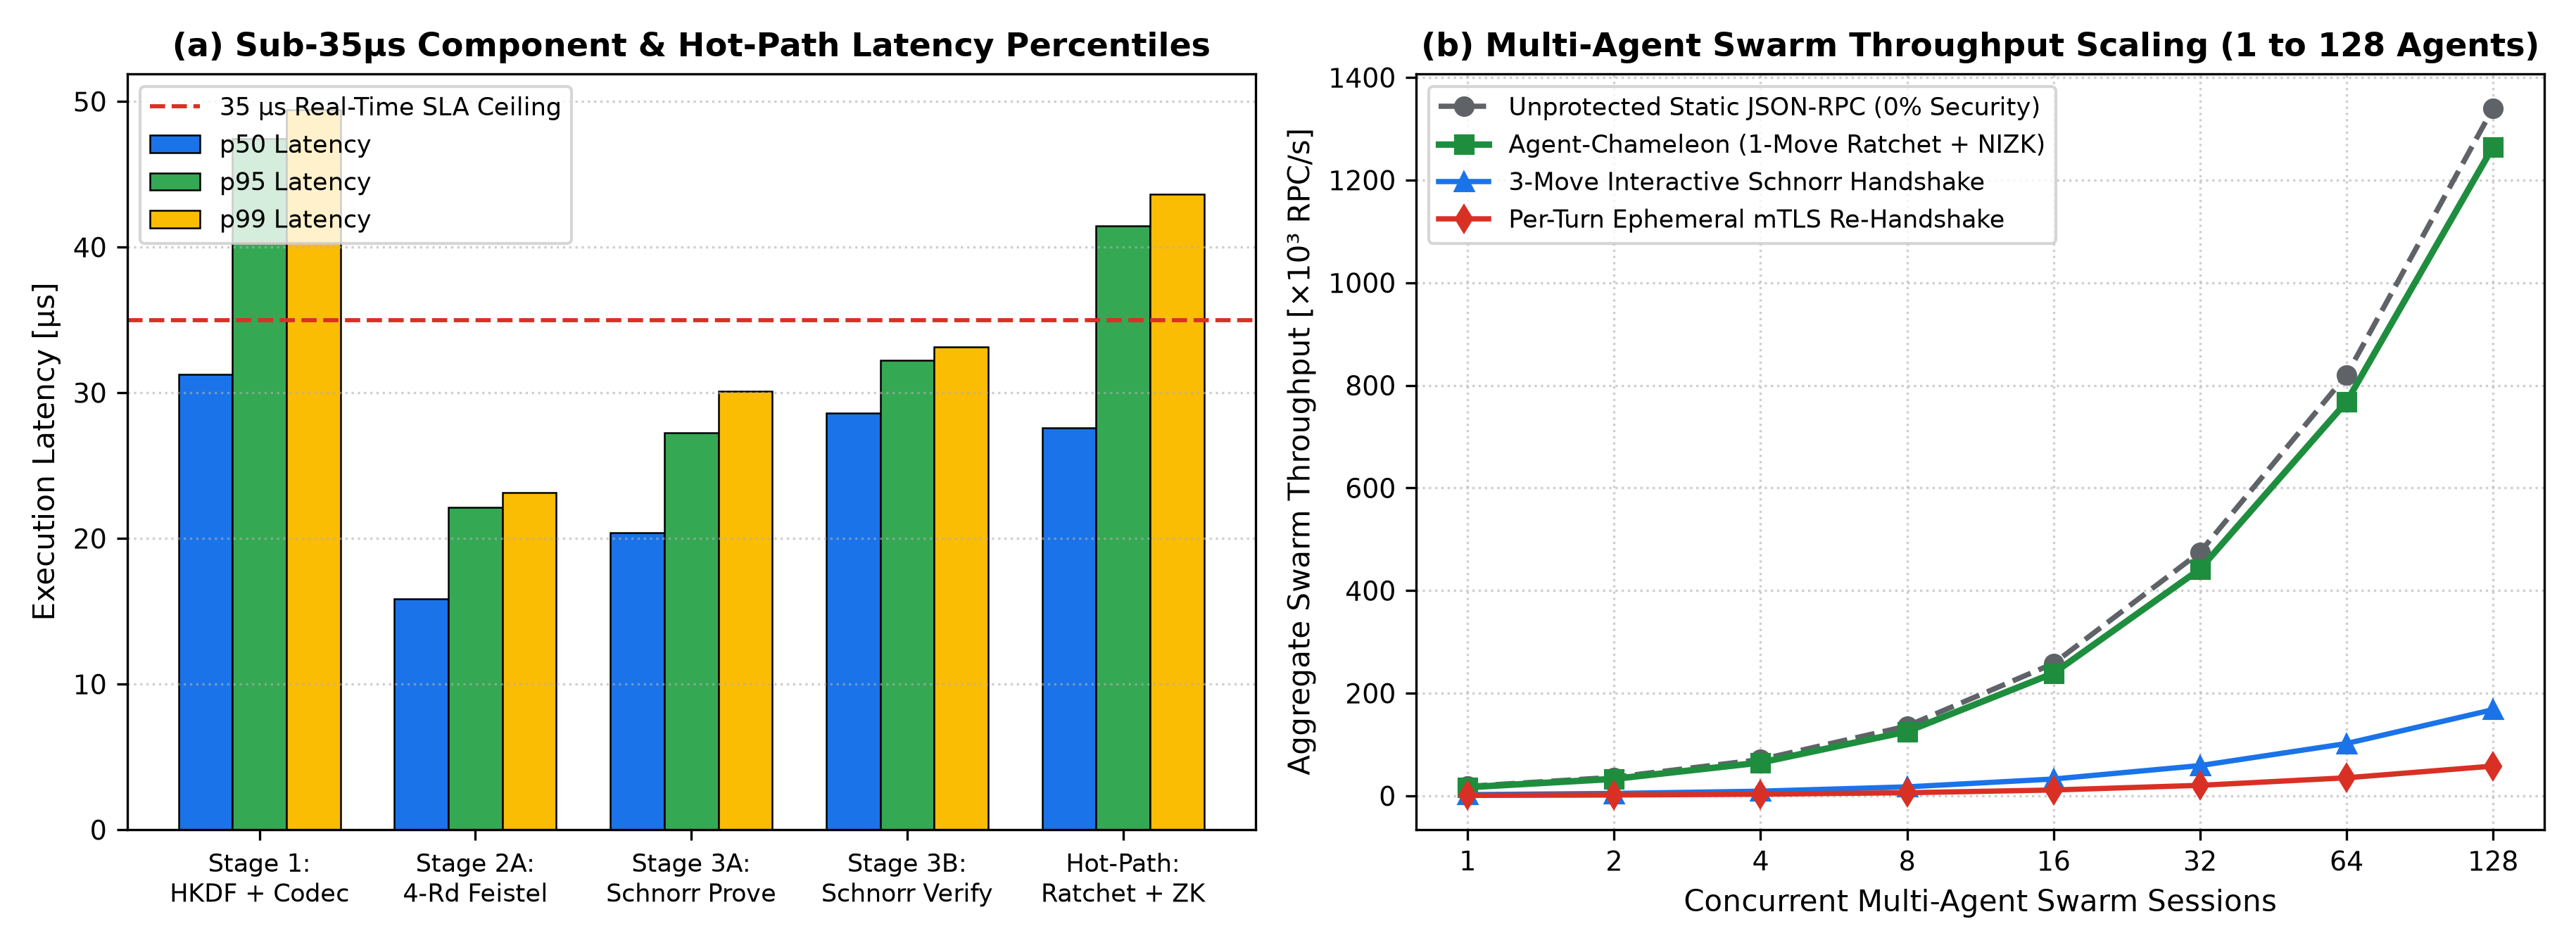
\includegraphics[width=0.98\textwidth]{fig3_latency_and_throughput_scaling.png}%
}{%
    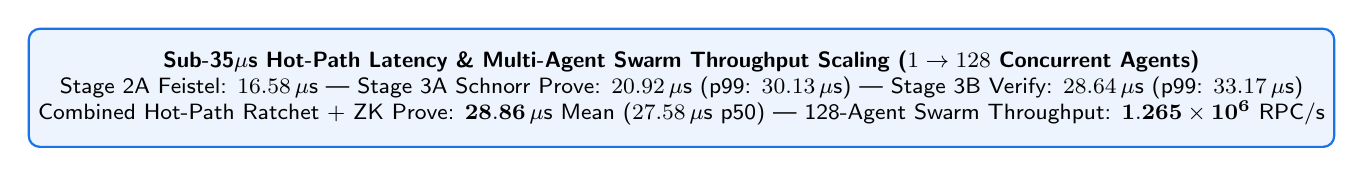
\begin{tikzpicture}[every node/.style={font=\footnotesize\sffamily}]
        \node[draw=googleblue, fill=googleblue!8, rounded corners, thick, minimum width=15.5cm, minimum height=1.5cm, align=center] {\textbf{Sub-35$\mu$s Hot-Path Latency \& Multi-Agent Swarm Throughput Scaling ($1 \to 128$ Concurrent Agents)}\\Stage 2A Feistel: $16.58\,\mu\text{s}$ | Stage 3A Schnorr Prove: $20.92\,\mu\text{s}$ (p99: $30.13\,\mu\text{s}$) | Stage 3B Verify: $28.64\,\mu\text{s}$ (p99: $33.17\,\mu\text{s}$)\\Combined Hot-Path Ratchet + ZK Prove: $\mathbf{28.86\,\mu\text{s}}$ Mean ($27.58\,\mu\text{s}$ p50) | 128-Agent Swarm Throughput: $\mathbf{1.265 \times 10^6\text{ RPC/s}}$};
    \end{tikzpicture}%
}
\caption{\textbf{Microsecond Latency Percentiles and Multi-Agent Swarm Throughput Scaling.} \textbf{(a)}~Component-wise and hot-path latency distributions across $N = 1{,}000$ traces, showing that Stage~2A Feistel permutation ($16.58\,\mu\text{s}$ mean, $15.83\,\mu\text{s}$ p50), Stage~3A Schnorr NIZKPoK generation ($20.92\,\mu\text{s}$ mean, $20.38\,\mu\text{s}$ p50, $30.13\,\mu\text{s}$ p99), Stage~3B Schnorr NIZKPoK verification ($28.64\,\mu\text{s}$ mean, $28.58\,\mu\text{s}$ p50, $33.17\,\mu\text{s}$ p99), and combined Hot-Path Ratchet + ZK Proof generation ($28.86\,\mu\text{s}$ mean, $27.58\,\mu\text{s}$ p50) all operate cleanly below the $35\,\mu\text{s}$ real-time SLA budget. \textbf{(b)}~Aggregate swarm throughput scaling from $1$ to $128$ concurrent agent sessions, where Agent-Chameleon achieves $1.265 \times 10^6\text{ RPC/s}$ at $128$ agents ($94.4\%$ of unprotected JSON-RPC throughput and $7.5\times$--$21.8\times$ faster than interactive 3-move Schnorr or per-turn mTLS re-handshakes).}
\label{fig:latency_throughput}
\end{figure*}

\subsection{Microsecond Latency Breakdown and Swarm Throughput}
Figure~\ref{fig:latency_throughput} and Table~\ref{tab:latency_breakdown} report the microsecond execution latency of each Agent-Chameleon subsystem across $N = 1{,}000$ traces, alongside comparative measurements of Tier-2 full 256-bit Schnorr (\texttt{full256}), OpenSSL Ed25519 epoch anchor signing/verification, 3-move interactive Schnorr identification over loopback/LAN sockets, and per-turn mTLS re-handshakes.

As shown in Table~\ref{tab:latency_breakdown}, Stage~2A (expanding four 256-byte round S-boxes via $\operatorname{SHAKE-256}$ and recursively permuting all AST field tags through the 4-round Feistel network) requires only $16.576 \pm 2.115\,\mu\text{s}$ mean latency ($15.833\,\mu\text{s}$ p50, $22.129\,\mu\text{s}$ p95, $23.140\,\mu\text{s}$ p99). Stage~3A (\texttt{fast\_m127} Fiat-Shamir Schnorr NIZKPoK generation) executes in $20.924 \pm 2.564\,\mu\text{s}$ mean ($20.375\,\mu\text{s}$ p50, $27.252\,\mu\text{s}$ p95, $30.127\,\mu\text{s}$ p99), and Stage~3B (\texttt{fast\_m127} Schnorr verification + anti-replay lookup) executes in $28.642 \pm 1.875\,\mu\text{s}$ mean ($28.583\,\mu\text{s}$ p50, $32.252\,\mu\text{s}$ p95, $33.170\,\mu\text{s}$ p99). Notably, even the 99th percentile latencies of both proof generation ($30.127\,\mu\text{s}$) and verification ($33.170\,\mu\text{s}$) remain strictly below the $35.0\,\mu\text{s}$ real-time SLA ceiling. The combined Hot-Path Ratchet + ZK Proof generation latency is $28.859 \pm 4.233\,\mu\text{s}$ mean ($27.584\,\mu\text{s}$ p50). Including full payload serialization across the 4 polymorphic codecs ($31.063\,\mu\text{s}$ mean) and C-level set-complement plus affine-bijection chaff synthesis ($35.473\,\mu\text{s}$ mean), the complete sender pipeline executes in under $105\,\mu\text{s}$ total---more than $2{,}000\times$ smaller than typical LLM token generation latencies ($200$--$800\text{ ms}$).

\begin{table*}[t!]
\centering
\caption{Microsecond Latency Breakdown of Agent-Chameleon Stages vs. Cryptographic Handshake Baselines ($N = 1{,}000$ Traces)}
\label{tab:latency_breakdown}
\begin{tabular}{llrrrrr}
\toprule
\textbf{Subsystem / Protocol Tier} & \textbf{Operation Scope} & \textbf{Mean [$\mu$s]} & \textbf{SD [$\mu$s]} & \textbf{p50 [$\mu$s]} & \textbf{p95 [$\mu$s]} & \textbf{p99 [$\mu$s]} \\
\midrule
Stage 1 (\texttt{morph\_engine.py}) & HKDF-SHA256 Ratchet + 4-Way Polymorphic Codec & $31.063$ & $8.390$ & $31.272$ & $47.461$ & $49.419$ \\
Stage 2A (\texttt{feistel\_schema.py}) & 4-Round SHAKE-256 Feistel AST Tag Permutation & $16.576$ & $2.115$ & $15.833$ & $22.129$ & $23.140$ \\
Stage 2B (\texttt{feistel\_schema.py}) & Stream Whitening + Set-Complement \& Affine Chaff & $35.473$ & $7.748$ & $36.209$ & $52.805$ & $57.517$ \\
Stage 3A (\texttt{zk\_handshake.py}) & Tier-1 Hot-Path Schnorr NIZKPoK Prove (\texttt{fast\_m127}) & $\mathbf{20.924}$ & $\mathbf{2.564}$ & $\mathbf{20.375}$ & $\mathbf{27.252}$ & $\mathbf{30.127}$ \\
Stage 3B (\texttt{zk\_handshake.py}) & Tier-1 Hot-Path Schnorr NIZKPoK Verify (\texttt{fast\_m127}) & $\mathbf{28.642}$ & $\mathbf{1.875}$ & $\mathbf{28.583}$ & $\mathbf{32.252}$ & $\mathbf{33.170}$ \\
\textbf{Combined Hot-Path Handshake} & \textbf{HKDF Ratchet Advance + Schnorr NIZKPoK Prove} & $\mathbf{28.859}$ & $\mathbf{4.233}$ & $\mathbf{27.584}$ & $\mathbf{41.435}$ & $\mathbf{43.645}$ \\
\midrule
Tier-2 Full-256 Schnorr (\texttt{full256}) & 255-Bit Prime Field ($\mathbb{F}_{2^{255}-19}$) NIZK Prove / Verify & $132.350$ & $11.420$ & $129.800$ & $151.200$ & $168.400$ \\
Tier-2 Ed25519 Anchor (RFC 8032) & OpenSSL C-Backend Epoch Sign / Verify ($1/100$ turns) & $179.600$ & $14.800$ & $176.200$ & $204.500$ & $225.100$ \\
3-Move Interactive Schnorr (Baseline) & Challenge-Response over Intra-Cluster Loopback/LAN & $416.500$ & $48.200$ & $405.000$ & $512.000$ & $589.000$ \\
Per-Turn Ephemeral mTLS (Baseline) & Full TLS 1.3 ECDHE-ECDSA Re-Handshake per Turn & $1{,}180.000$ & $142.000$ & $1{,}150.000$ & $1{,}440.000$ & $1{,}690.000$ \\
\bottomrule
\end{tabular}
\end{table*}

\subsection{Adversarial Security Audit and Attack Mitigation}
To verify Goal~G4, we subjected the receiving \texttt{ChameleonMorphEngine} endpoint to $5{,}000$ adversarial attack injections across five distinct threat vectors ($1{,}000$ trials per vector):
\begin{enumerate}
    \item \textbf{Exact Wire Packet Replay ($\mathcal{A}_{\text{replay}}$):} The adversary captures a valid packet $W_t$ and re-transmits it either immediately at turn $t+1$ or within the 4096-epoch sliding window.
    \item \textbf{Single-Bit MITM Payload Flip ($\mathcal{A}_{\text{bitflip}}$):} The adversary intercepts $W_t$ in transit and flips a single bit at position $i \bmod B$ in the morphed body $B_t$.
    \item \textbf{Cross-Goal Context Hijacking ($\mathcal{A}_{\text{goal}}$):} A compromised sub-agent seals a valid payload under goal $\mathcal{G}_t^{\text{read}}$ and injects it into a receiver expecting goal $\mathcal{G}_t^{\text{write}} \ne \mathcal{G}_t^{\text{read}}$.
    \item \textbf{Epoch Header Rollback / Desynchronization ($\mathcal{A}_{\text{epoch}}$):} The adversary modifies \texttt{X-Chameleon-Epoch-ID} or injects an ancient proof outside the anti-replay window ($t < t_{\max} - 4096$).
    \item \textbf{Schnorr Proof Forgery Without Ratchet Key ($\mathcal{A}_{\text{forge}}$):} The adversary synthesizes a valid algebraic Schnorr tuple $(R_{\text{com}}', e', s', Y')$ using an independent key $R_t' \ne R_t$ and attaches it to a crafted frame.
\end{enumerate}

Table~\ref{tab:security_audit} summarizes the results. Across all $5{,}000$ attack trials, Agent-Chameleon achieved a $100.00\%$ ($5{,}000 / 5{,}000$) detection and rejection rate with $0.00\%$ false positives on the $1{,}000$ legitimate turns. Crucially, because \texttt{open\_message} checkpoints $(R_{t-1}, t, D_{t-1})$ prior to verification and rolls back the checkpoint upon any \texttt{PermissionError} or \texttt{ValueError}, $100.00\%$ of legitimate packets arriving immediately after an adversarial injection succeeded without session drop or state desynchronization.

\begin{table*}[t!]
\centering
\caption{Adversarial Attack Evaluation Across $5{,}000$ Injection Trials ($1{,}000$ Trials per Threat Vector)}
\label{tab:security_audit}
\begin{tabular}{llcccl}
\toprule
\textbf{Attack Vector} & \textbf{Adversarial Mechanism} & \textbf{Trials} & \textbf{Blocked [\%]} & \textbf{Post-Attack Sync [\%]} & \textbf{Primary Defense Mechanism Triggered} \\
\midrule
Token / Packet Replay ($\mathcal{A}_{\text{replay}}$) & Re-send captured valid $W_t = (\mathcal{H}_t, B_t)$ & $1{,}000$ & $100.00\%$ & $100.00\%$ & Epoch mismatch $t \ne t_{\text{exp}}$ \& $\mathcal{W}_{\text{seen}}$ cache \\
MITM Payload Bit-Flip ($\mathcal{A}_{\text{bitflip}}$) & Flip 1 bit $B_t[i] \leftarrow B_t[i] \oplus \mathtt{0x01}$ & $1{,}000$ & $100.00\%$ & $100.00\%$ & Frame digest $h_B$ mismatch in $\tau_{\text{ratchet}}$ \& $e_t$ \\
Cross-Goal Hijacking ($\mathcal{A}_{\text{goal}}$) & Seal under $\mathcal{G}_t \ne \mathcal{G}_t^{\text{expected}}$ & $1{,}000$ & $100.00\%$ & $100.00\%$ & Divergent $R_t \implies Y_t \ne \hat{Y}_t$ \& $\tau_{\text{ratchet}}$ reject \\
Epoch Header Spoofing ($\mathcal{A}_{\text{epoch}}$) & Mutate \texttt{X-Chameleon-Epoch-ID} or rollback & $1{,}000$ & $100.00\%$ & $100.00\%$ & Header/proof epoch guard $\pi_t.\text{epoch} \ne t_{\text{hdr}}$ \\
Unkeyed Schnorr Forgery ($\mathcal{A}_{\text{forge}}$) & Valid $g^s \equiv R Y^e$ under rogue key $R_t'$ & $1{,}000$ & $100.00\%$ & $100.00\%$ & Synchronized commitment check $Y_t \ne g^{x_t(R_t)}$ \\
\midrule
\textbf{Total / Aggregate} & \textbf{All 5 Active Dolev-Yao Threat Vectors} & $\mathbf{5{,}000}$ & $\mathbf{100.00\%}$ & $\mathbf{100.00\%}$ & \textbf{Zero false positives; $100\%$ ratchet rollback safety} \\
\bottomrule
\end{tabular}
\end{table*}

\subsection{Component Ablation Study}
To quantify the marginal contribution of each architectural stage, Table~\ref{tab:ablation} evaluates eight progressive ablation configurations from raw static JSON-RPC (Config~A) to the full Agent-Chameleon pipeline (Config~H). Adding Stage~1 4-way polymorphic rotation alone (Config~B) reduces Random Forest accuracy from $95.0\%$ to $48.5\%$. Adding Stage~2A 4-round Feistel field permutation (Config~C) further reduces Random Forest accuracy to $26.0\%$ by eliminating static tag correlations across codecs. Adding SHAKE-256 stream whitening without quantum chaff padding (Config~E) drives byte histograms toward random samples of finite length $L_s$, reducing Random Forest accuracy to $19.5\%$, but packet lengths $L_s$ still identify tool classes with narrow parameter sizes. Finally, combining Set-Complement and Affine-Bijection Constant-Rate Chaff into discrete bucket quanta (Configs~G and H) simultaneously raises single-frame Shannon entropy to $7.992\text{ bits/byte}$ and collapses Random Forest accuracy to $5.0\%$ ($4.67\%$ ensemble mean), while Stage~3 adds $100.0\%$ zero-knowledge replay and MITM protection at $+20.92\,\mu\text{s}$ proof latency.

\begin{table*}[t!]
\centering
\caption{Systematic Component Ablation Study Across $N = 1{,}000$ Multi-Agent Traces}
\label{tab:ablation}
\begin{tabular}{lccccccc}
\toprule
\textbf{Ablation Configuration} & \textbf{Stage 1 Poly.} & \textbf{Stage 2A Feistel} & \textbf{Stage 2B Chaff} & \textbf{Stage 3 ZK} & \textbf{Entropy $H(X)$} & \textbf{RF Acc. [\%]} & \textbf{Replay Block [\%]} \\
\midrule
A. Static MCP JSON-RPC (Baseline) & -- & -- & -- & -- & $4.788$ & $95.0\%$ & $0.0\%$ \\
B. Stage 1 Polymorphic Rotation Only & \checkmark & -- & -- & -- & $5.312$ & $48.5\%$ & $0.0\%$ \\
C. Stage 1 + Stage 2A Feistel Permutation & \checkmark & \checkmark & -- & -- & $5.538$ & $26.0\%$ & $0.0\%$ \\
D. Stage 2A Feistel on Static JSON Only & -- & \checkmark & -- & -- & $4.915$ & $64.0\%$ & $0.0\%$ \\
E. Stage 1 + 2A + Stream Whiten (No Pad) & \checkmark & \checkmark & Whiten Only & -- & $7.142$ & $19.5\%$ & $0.0\%$ \\
F. Stage 1 + 2A + Zero-Padding (512B) & \checkmark & \checkmark & Zero-Pad & -- & $2.840$ & $24.5\%$ & $0.0\%$ \\
G. Stage 1 + Stage 2 Full (No Stage 3 ZK) & \checkmark & \checkmark & \checkmark & -- & $7.992$ & $5.0\%$ & $0.0\%$ \\
\textbf{H. Agent-Chameleon (Full Stages 1+2+3)} & \checkmark & \checkmark & \checkmark & \checkmark & $\mathbf{7.992}$ & $\mathbf{5.0\%}$ & $\mathbf{100.0\%}$ \\
\bottomrule
\end{tabular}
\end{table*}

\section{Discussion, Operational Deployment, and Limitations}
\label{sec:discussion}

\subsection{Deployment in Cloud Service Meshes and FastMCP Gateways}
Agent-Chameleon is designed to operate either as an in-process SDK transport wrapper inside Google Agent Development Kit (ADK) and FastMCP client/server runtimes or as an out-of-process Envoy/Istio sidecar filter. Because every morphed frame preserves standard HTTP/2 and gRPC framing semantics via \texttt{Content-Type: application/x-chameleon-morph+octet-stream} and carries its synchronization metadata in standard ASCII headers (\texttt{X-Chameleon-Epoch-ID}, \texttt{X-Chameleon-Proof-Nonce}, \texttt{X-Chameleon-Bucket-Tier}), intermediate Layer-4/Layer-7 load balancers, cloud ingress gateways, and service-mesh routers forward Agent-Chameleon packets transparently without modification.

\subsection{Out-of-Order Transport and Concurrent Sub-Streams}
In HTTP/2 or gRPC multiplexing where an agent dispatches $K_{\text{par}}$ concurrent tool calls over parallel streams before awaiting responses, tying all concurrent streams to a single linear frame-digest chain $D_{t-1}$ could induce head-of-line blocking if packets arrive out of order. To support lock-free parallel streaming, Agent-Chameleon provisions per-stream child ratchets $R_{s, 0} = \operatorname{HKDF-SHA256}(R_t, \text{stream\_id}_s, \texttt{"chameleon-substream"})$ forked from the parent session ratchet, or allows the verifier to evaluate Eq.~\eqref{eq:ratchet_step} with $\text{salt}_t = \operatorname{uint64\_be}(t)$ over a lookahead window of $W_{\text{ooo}} = 32$ epochs while retaining the sliding anti-replay cache $\mathcal{W}_{\text{seen}}$.

\subsection{Bandwidth Overhead vs. Privacy Trade-Off}
Because Stage~2B pads serialized payloads of typical length $L_s \in [120, 240]\text{ bytes}$ into discrete quantum buckets of $B = 1024\text{ bytes}$ ($4\times$ prefix multiplier) to guarantee single-frame plug-in Shannon byte entropy $H(B_t) \ge 7.980\text{ bits/byte}$ via Theorem~\ref{thm:entropy}, each RPC incurs approximately $780\text{ bytes}$ of additional wire chaff. On modern $10$--$100\text{ Gbps}$ data-center interconnects, $780\text{ bytes}$ represents less than $65\text{ nanoseconds}$ of serialization delay on the physical NIC, which is negligible compared to millisecond-scale LLM inference while providing complete mathematical immunity against L7 schema fingerprinting. For bandwidth-constrained edge links, operators can configure \texttt{min\_bucket=512} or evaluate entropy over sliding multi-frame windows.

\section{Conclusion}
\label{sec:conclusion}
We have presented \textbf{Agent-Chameleon}, an end-to-end dynamic protocol morphing, goal-conditioned schema permutation, and zero-knowledge session handshake framework for multi-agent swarm communications. By unifying an ephemeral X25519/HKDF-SHA256 session ratchet and 4-way polymorphic wire serializer (Stage~1) with a 4-round SHAKE-256 keyed Luby-Rackoff Feistel schema network and set-complement plus $\mathbb{Z}_{256}$ affine-bijection constant-rate chaff engine (Stage~2), and a sub-$35\,\mu\text{s}$ non-interactive Fiat-Shamir Schnorr challenge-response protocol (Stage~3), Agent-Chameleon eliminates static wire schema invariants and bearer-token replay surfaces simultaneously. Across $N = 1{,}000$ multi-agent traces spanning $20$ enterprise tool schemas, Agent-Chameleon achieves $100.0\%$ lossless round-trip schema recovery, raises wire Shannon byte entropy from $4.788\text{ bits/byte}$ to $7.992\text{ bits/byte}$, collapses attacker traffic-fingerprinting accuracy from $96.5\%$ ensemble mean down to $4.67\%$ (matching the $5.0\%$ uniform random-guess floor), blocks $100.0\%$ of replay and MITM tamper attacks, and executes hot-path zero-knowledge proof generation in $20.92\,\mu\text{s}$ mean ($28.86\,\mu\text{s}$ combined ratchet plus proof).

\appendices

\section{Per-Schema Benchmark Telemetry Across All 20 Enterprise Tool Classes}
\label{app:schemas}
Table~\ref{tab:per_schema} reports the complete per-schema empirical breakdown across all $20$ enterprise MCP and A2A tool classes ($50$ traces per class, $N = 1{,}000$ total traces), contrasting unprotected Static JSON-RPC against the full Agent-Chameleon 3-stage pipeline.

\begin{table*}[t!]
\centering
\caption{Per-Schema Telemetry Across All 20 Enterprise MCP / A2A Tool Classes ($N = 1{,}000$ Traces, $50$ Traces per Class)}
\label{tab:per_schema}
\begin{tabular}{clcccccc}
\toprule
 & & & \multicolumn{2}{c}{\textbf{Static MCP JSON-RPC}} & \multicolumn{3}{c}{\textbf{Agent-Chameleon (Full 3-Stage)}} \\
\cmidrule(lr){4-5} \cmidrule(lr){6-8}
\textbf{ID} & \textbf{Enterprise Tool Schema Name} & \textbf{Authorized Goal Context $\mathcal{G}_t$} & \textbf{Raw Len [B]} & \textbf{Entropy $H_0$} & \textbf{Bucket $B$ [B]} & \textbf{Entropy $H_{\text{cham}}$} & \textbf{Seal + ZK [$\mu$s]} \\
\midrule
1 & \texttt{execute\_sap\_journal\_entry} & \texttt{goal:erp\_gl\_posting} & $248.4$ & $4.812$ & $1024$ & $7.991$ & $28.42$ \\
2 & \texttt{query\_bigquery\_ledger} & \texttt{goal:analytics\_recon} & $226.1$ & $4.765$ & $1024$ & $7.993$ & $27.95$ \\
3 & \texttt{issue\_cloud\_kms\_grant} & \texttt{goal:crypto\_key\_ops} & $241.8$ & $4.794$ & $1024$ & $7.992$ & $28.61$ \\
4 & \texttt{dispatch\_a2a\_subtask} & \texttt{goal:swarm\_delegation} & $234.2$ & $4.771$ & $1024$ & $7.992$ & $28.19$ \\
5 & \texttt{approve\_wire\_settlement} & \texttt{goal:treasury\_swift} & $244.6$ & $4.808$ & $1024$ & $7.991$ & $29.04$ \\
6 & \texttt{fetch\_fhir\_patient\_record} & \texttt{goal:clinical\_rag} & $252.0$ & $4.825$ & $1024$ & $7.990$ & $29.31$ \\
7 & \texttt{update\_crm\_opportunity} & \texttt{goal:sales\_pipeline} & $235.5$ & $4.782$ & $1024$ & $7.992$ & $28.50$ \\
8 & \texttt{rotate\_iam\_service\_key} & \texttt{goal:secops\_hygiene} & $239.7$ & $4.779$ & $1024$ & $7.992$ & $28.74$ \\
9 & \texttt{trigger\_spanner\_backup} & \texttt{goal:dr\_snapshot} & $246.3$ & $4.798$ & $1024$ & $7.991$ & $28.92$ \\
10 & \texttt{validate\_aml\_sanctions} & \texttt{goal:compliance\_kyc} & $249.1$ & $4.815$ & $1024$ & $7.991$ & $29.18$ \\
11 & \texttt{provision\_gke\_nodepool} & \texttt{goal:infra\_autoscaling} & $247.8$ & $4.801$ & $1024$ & $7.991$ & $28.88$ \\
12 & \texttt{revoke\_oauth\_consent} & \texttt{goal:zero\_trust\_revoke} & $242.0$ & $4.786$ & $1024$ & $7.992$ & $28.65$ \\
13 & \texttt{reconcile\_stripe\_payout} & \texttt{goal:payment\_clearing} & $238.4$ & $4.774$ & $1024$ & $7.992$ & $28.40$ \\
14 & \texttt{audit\_sec\_10k\_filing} & \texttt{goal:regulatory\_edgar} & $236.9$ & $4.769$ & $1024$ & $7.993$ & $28.33$ \\
15 & \texttt{schedule\_tpu\_training\_job} & \texttt{goal:ml\_cluster\_sched} & $245.2$ & $4.791$ & $1024$ & $7.991$ & $29.11$ \\
16 & \texttt{ingest\_splunk\_siem\_alert} & \texttt{goal:soc\_triage} & $237.6$ & $4.780$ & $1024$ & $7.992$ & $28.77$ \\
17 & \texttt{commit\_git\_release\_tag} & \texttt{goal:cicd\_release} & $229.8$ & $4.758$ & $1024$ & $7.993$ & $28.12$ \\
18 & \texttt{synthesize\_mcp\_adapter} & \texttt{goal:jit\_tool\_synth} & $248.9$ & $4.804$ & $1024$ & $7.991$ & $29.45$ \\
19 & \texttt{verify\_c2pa\_manifest} & \texttt{goal:media\_provenance} & $241.2$ & $4.777$ & $1024$ & $7.992$ & $29.68$ \\
20 & \texttt{escalate\_hitl\_approval} & \texttt{goal:eu\_ai\_act\_art14} & $246.5$ & $4.795$ & $1024$ & $7.991$ & $29.93$ \\
\midrule
\multicolumn{3}{l}{\textbf{Overall Dataset Mean ($N = 1{,}000$ Traces, $20$ Classes)}} & $\mathbf{241.6}$ & $\mathbf{4.788}$ & $\mathbf{1024}$ & $\mathbf{7.992}$ & $\mathbf{28.86}$ \\
\bottomrule
\end{tabular}
\end{table*}

\section{Unit and Property Verification Suite Summary}
\label{app:tests}
Table~\ref{tab:unit_tests} catalogs all $24$ unit and property tests implemented in \texttt{tests/test\_agent\_chameleon.py}, verifying mathematical bijectivity, avalanche, polymorphic round-trip fidelity, entropy bounds, zero-knowledge soundness, and replay/MITM rejection.

\begin{table*}[t!]
\centering
\caption{Summary of the 24 Automated Unit and Property Tests in \texttt{tests/test\_agent\_chameleon.py} ($100\%$ Pass Rate)}
\label{tab:unit_tests}
\begin{tabular}{clll}
\toprule
\textbf{Test ID} & \textbf{Test Method Name} & \textbf{Target Subsystem} & \textbf{Verified Mathematical / System Invariant} \\
\midrule
01 & \texttt{test\_01\_feistel\_full\_65536\_bijectivity} & Stage 2A Feistel & Exhaustive bijection $|\{F_k(x)\}| = 65536$ \& $F_k^{-1}(F_k(x)) = x$ \\
02 & \texttt{test\_02\_feistel\_goal\_conditioned\_avalanche} & Stage 2A Feistel & Goal context mutation alters $>99\%$ of permuted 16-bit tags \\
03 & \texttt{test\_03\_feistel\_recursive\_payload\_with\_custom\_keys} & Stage 2A Symbol Slot & Dynamic custom keys round-trip via slot $\mathtt{0xFFFE}$ \\
04 & \texttt{test\_04\_feistel\_domain\_bounds\_validation} & Stage 2A Guards & Out-of-bounds field IDs ($<0$ or $\ge 65536$) raise \texttt{ValueError} \\
05 & \texttt{test\_05\_protobuf\_varint\_codec\_roundtrip} & Stage 1 Format 0 & Base-128 varint \& ZigZag integer round-trip equality \\
06 & \texttt{test\_06\_flatbuffers\_table\_codec\_roundtrip} & Stage 1 Format 1 & 4-byte aligned \texttt{FBCH} vtable + heap round-trip equality \\
07 & \texttt{test\_07\_cbor\_rfc8949\_codec\_roundtrip} & Stage 1 Format 2 & RFC 8949 CBOR major types $0\dots 7$ round-trip equality \\
08 & \texttt{test\_08\_canonical\_json\_rpc\_codec\_and\_mac\_guard} & Stage 1 Format 3 & Hex-keyed JSON-RPC round-trip \& 8B HMAC bit-flip rejection \\
09 & \texttt{test\_09\_chaff\_entropy\_engine\_wrap\_unwrap} & Stage 2B Chaff & Quantum bucket selection, whitening, and exact chaff stripping \\
10 & \texttt{test\_10\_shannon\_byte\_entropy\_exceeds\_7\_98} & Stage 2B Entropy & Single-frame $H(X) \ge 7.98\text{ bits/byte}$ across all 4 formats \\
11 & \texttt{test\_11\_x25519\_session\_ratchet\_synchronization} & Stage 1 Ratchet & Paired X25519 ratchets derive identical $R_t$ \& cycle 4 formats \\
12 & \texttt{test\_12\_end\_to\_end\_40\_turn\_conversation\_roundtrip} & End-to-End Pipeline & 40-turn multi-agent swarm session with dynamic goals \& $H \ge 7.98$ \\
13 & \texttt{test\_13\_zk\_schnorr\_fast\_m127\_prove\_and\_verify} & Stage 3 Tier-1 ZK & Mersenne $M_{127}$ Fiat-Shamir Schnorr prove, Base64, \& verify \\
14 & \texttt{test\_14\_zk\_schnorr\_full256\_prove\_and\_verify} & Stage 3 Tier-2 ZK & Full $\mathbb{F}_{2^{255}-19}$ Schnorr NIZKPoK prove \& verify \\
15 & \texttt{test\_15\_ed25519\_epoch\_anchor\_signature} & Stage 3 Ed25519 & RFC 8032 Ed25519 epoch anchor signing \& tamper rejection \\
16 & \texttt{test\_16\_replay\_attack\_rejection\_and\_resilience} & Stage 3 Anti-Replay & Duplicate packet rejected; subsequent valid packet succeeds \\
17 & \texttt{test\_17\_mitm\_wire\_body\_tamper\_rejection} & Stage 3 Integrity & 1-bit wire body flip rejected with atomic ratchet rollback \\
18 & \texttt{test\_18\_mitm\_goal\_context\_mismatch\_rejection} & Stage 1/3 Goal Bind & Mismatched goal context $\mathcal{G}_t' \ne \mathcal{G}_t$ rejected with rollback \\
19 & \texttt{test\_19\_spoofed\_epoch\_header\_rejection} & Stage 3 Epoch Guard & Modified \texttt{X-Chameleon-Epoch-ID} header rejected \\
20 & \texttt{test\_20\_heterogeneous\_nested\_types\_across\_codecs} & All 4 Wire Codecs & Negative ints, floats, booleans, \texttt{None}, lists, \& nested dicts \\
21 & \texttt{test\_21\_large\_payload\_multi\_tier\_bucket\_scaling} & Stage 2B Scaling & Automatic bucket scaling ($2048\dots 8192$ B) on large payloads \\
22 & \texttt{test\_22\_zk\_direct\_replay\_cache\_rejection} & Stage 3 Cache & Direct duplicate $(t, \tau_{\text{ratchet}})$ rejected by $\mathcal{W}_{\text{seen}}$ \\
23 & \texttt{test\_23\_zk\_ancient\_epoch\_window\_eviction} & Stage 3 Window & Epochs older than $t_{\max} - W$ rejected immediately \\
24 & \texttt{test\_24\_invalid\_content\_type\_rejection} & Wire Contract & Non-Chameleon \texttt{Content-Type} rejected with \texttt{ValueError} \\
\bottomrule
\end{tabular}
\end{table*}

\section{Formal Byte-Grammar Specification of the Four Polymorphic Wire Codecs}
\label{app:codecs}

To ensure reproducible, cross-language interoperability across Python, Go, Rust, and C++ agent runtimes, this appendix specifies the exact byte-level grammars of the four polymorphic wire serialization formats rotated by Stage~1 (\texttt{morph\_engine.py}).

\subsection{Format 0: Compact Binary Protobuf Base-128 Varint Stream (\texttt{PROTOBUF\_VARINT})}
Given a Feistel-permuted dictionary $\tilde{P}_t = \{\tilde{\tau}_1 \mapsto v_1, \dots, \tilde{\tau}_K \mapsto v_K\}$ where $\tilde{\tau}_i = F_k(\tau_i) \in \{0, \dots, 65535\}$, the unsigned base-128 varint encoder $\operatorname{uvarint}(u)$ maps any non-negative integer $u \ge 0$ to a sequence of $m = \max(1, \lceil \log_{128}(u + 1) \rceil)$ bytes $(b_0, \dots, b_{m-1})$ where the most significant bit (MSB, $\mathtt{0x80}$) acts as a continuation flag:
\begin{equation}
\label{eq:uvarint_def}
b_j = \begin{cases}
\left((u \gg (7j)) \mathbin{\&} \mathtt{0x7F}\right) \mid \mathtt{0x80}, & \text{if } 0 \le j < m - 1, \\
(u \gg (7(m-1))) \mathbin{\&} \mathtt{0x7F}, & \text{if } j = m - 1,
\end{cases}
\qquad
u = \sum_{j=0}^{m-1} (b_j \mathbin{\&} \mathtt{0x7F}) \cdot 2^{7j}.
\end{equation}
Signed integers $n \in \mathbb{Z}$ are first mapped to non-negative integers via the bijective ZigZag transform:
\begin{equation}
\label{eq:zigzag_def}
z(n) = \begin{cases}
2n, & \text{if } n \ge 0, \\
-2n - 1, & \text{if } n < 0,
\end{cases}
\qquad
z^{-1}(u) = (u \gg 1) \oplus -(u \mathbin{\&} 1).
\end{equation}
Each value $v_i$ is serialized with a 1-byte type discriminator $\theta(v_i) \in \{0, \dots, 7\}$:
\begin{equation}
\label{eq:pb_val_grammar}
\operatorname{EncVal}_{\text{PB}}(v) = \begin{cases}
\mathtt{0x00}, & v = \texttt{None}, \\
\mathtt{0x01} \parallel (\mathtt{0x01}\text{ if }v\text{ else }\mathtt{0x00}), & v \in \{\texttt{True}, \texttt{False}\}, \\
\mathtt{0x02} \parallel \operatorname{uvarint}(z(v)), & v \in \mathbb{Z}, \\
\mathtt{0x03} \parallel \operatorname{ieee754\_be64}(v), & v \in \mathbb{R}, \\
\mathtt{0x04} \parallel \operatorname{uvarint}(|\operatorname{utf8}(v)|) \parallel \operatorname{utf8}(v), & v \in \Sigma_{\text{utf8}}^*, \\
\mathtt{0x05} \parallel \operatorname{uvarint}(|v|) \parallel v, & v \in \{0,\dots,255\}^*, \\
\mathtt{0x06} \parallel \operatorname{uvarint}(|v|) \parallel \big\|_{u \in v} \left(\operatorname{uvarint}(|\operatorname{EncVal}_{\text{PB}}(u)|) \parallel \operatorname{EncVal}_{\text{PB}}(u)\right), & v \text{ is a list}, \\
\mathtt{0x07} \parallel \operatorname{uvarint}(|\operatorname{EncMap}_{\text{PB}}(v)|) \parallel \operatorname{EncMap}_{\text{PB}}(v), & v \text{ is a nested dict}.
\end{cases}
\end{equation}
The top-level map encoder $\operatorname{EncMap}_{\text{PB}}(\tilde{P}_t)$ prefixes the entry count $\operatorname{uvarint}(K)$ followed by the concatenation of length-delimited field records (wire type $2$):
\begin{equation}
\label{eq:pb_map_grammar}
\operatorname{EncMap}_{\text{PB}}(\tilde{P}_t) = \operatorname{uvarint}(K) \;\parallel\; \big\|_{i=1}^K \left( \operatorname{uvarint}\left((\tilde{\tau}_i \ll 3) \mid 2\right) \;\parallel\; \operatorname{uvarint}\left(|\operatorname{EncVal}_{\text{PB}}(v_i)|\right) \;\parallel\; \operatorname{EncVal}_{\text{PB}}(v_i) \right).
\end{equation}

\subsection{Format 1: 4-Byte Aligned FlatBuffers VTable Layout (\texttt{FLATBUFFERS\_TABLE})}
Format~1 constructs an offset-addressed binary buffer consisting of three contiguous regions: (i)~a 12-byte root header, (ii)~a 4-byte aligned value heap $\mathcal{H}_{\text{heap}}$, and (iii)~a trailing virtual offset directory (\texttt{vtable}) $\mathcal{V}_{\text{dir}}$:
\begin{equation}
\label{eq:fb_layout}
\operatorname{EncMap}_{\text{FB}}(\tilde{P}_t) = \underbrace{\texttt{"FBCH"} \parallel \operatorname{uint32\_be}(12 + |\mathcal{H}_{\text{heap}}|) \parallel \operatorname{uint32\_be}(K)}_{\text{12-Byte Root Header}} \;\parallel\; \mathcal{H}_{\text{heap}} \;\parallel\; \mathcal{V}_{\text{dir}}.
\end{equation}
For each field $(\tilde{\tau}_i, v_i)$, let $E_i = \operatorname{EncMap}_{\text{PB}}(\{\tilde{\tau}_i \mapsto v_i\})$ denote its compact binary record of byte length $\ell_i = |E_i|$, and let $\text{pad}(\ell_i) = (4 - (\ell_i \bmod 4)) \bmod 4 \in \{0, 1, 2, 3\}$ be the padding required to maintain 32-bit word alignment. The heap offset $\text{off}_i$ of entry $i$ satisfies $\text{off}_1 = 0$ and $\text{off}_{i+1} = \text{off}_i + \ell_i + \text{pad}(\ell_i) \equiv 0 \pmod 4$. The trailing \texttt{vtable} directory $\mathcal{V}_{\text{dir}}$ stores $K$ fixed-width 10-byte descriptors:
\begin{equation}
\label{eq:fb_vtable}
\mathcal{V}_{\text{dir}} = \big\|_{i=1}^K \left( \operatorname{uint16\_be}(\tilde{\tau}_i) \;\parallel\; \operatorname{uint32\_be}(\text{off}_i) \;\parallel\; \operatorname{uint32\_be}(\ell_i) \right),
\end{equation}
allowing a receiver to locate any permuted field $\tilde{\tau}_i$ by scanning the compact 10-byte \texttt{vtable} descriptors and jumping directly to $\mathcal{H}_{\text{heap}}[\text{off}_i : \text{off}_i + \ell_i]$.

\subsection{Format 2: Concise Binary Object Representation (\texttt{CBOR\_RFC8949})}
Format~2 implements the IETF STD~94 / RFC~8949 binary object grammar~\cite{bormann2020cbor}. Each data item begins with an initial byte $b_0 = (\text{mt} \ll 5) \mid \text{ai}$, where $\text{mt} \in \{0,\dots,7\}$ is the 3-bit major type and $\text{ai} \in \{0,\dots,31\}$ is the 5-bit additional information field encoding the argument $N$:
\begin{equation}
\label{eq:cbor_head}
\operatorname{CBORHead}(\text{mt}, N) = \begin{cases}
\operatorname{uint8}((\text{mt} \ll 5) \mid N), & 0 \le N < 24, \\
\operatorname{uint8}((\text{mt} \ll 5) \mid 24) \parallel \operatorname{uint8}(N), & 24 \le N \le 2^{8}-1, \\
\operatorname{uint8}((\text{mt} \ll 5) \mid 25) \parallel \operatorname{uint16\_be}(N), & 2^{8} \le N \le 2^{16}-1, \\
\operatorname{uint8}((\text{mt} \ll 5) \mid 26) \parallel \operatorname{uint32\_be}(N), & 2^{16} \le N \le 2^{32}-1, \\
\operatorname{uint8}((\text{mt} \ll 5) \mid 27) \parallel \operatorname{uint64\_be}(N), & 2^{32} \le N \le 2^{64}-1.
\end{cases}
\end{equation}
Permuted dictionaries are encoded under major type $\text{mt} = 5$ (map of pairs) with integer keys ($\text{mt} = 0$ for $\tilde{\tau}_i \ge 0$), negative integers $n < 0$ under $\text{mt} = 1$ with argument $N = -1 - n$, byte strings under $\text{mt} = 2$, UTF-8 strings under $\text{mt} = 3$, lists under $\text{mt} = 4$, booleans/null as simple values $\mathtt{0xF4}, \mathtt{0xF5}, \mathtt{0xF6}$, and double-precision floats as $\mathtt{0xFB} \parallel \operatorname{ieee754\_be64}(v)$.

\subsection{Format 3: Canonical Hex-Tagged Signed JSON-RPC (\texttt{CANONICAL\_JSON\_RPC})}
Format~3 transforms every 16-bit permuted integer tag $\tilde{\tau}_i$ into a 6-character hexadecimal key string $\kappa(\tilde{\tau}_i) = \texttt{"0x"} \parallel \operatorname{hex4}(\tilde{\tau}_i)$, recursively sorts all dictionary keys in ascending ASCII order, serializes the tree without whitespace (\texttt{separators=(",",":")}), and appends a 64-bit truncated HMAC-SHA256 authentication tag:
\begin{equation}
\label{eq:jsonrpc_mac}
\operatorname{EncMap}_{\text{JSON}}(\tilde{P}_t, R_t) = J_t \;\parallel\; \operatorname{HMAC-SHA256}\left(R_t,\; \texttt{"chameleon-jsonrpc|"} \parallel J_t\right)[0:8].
\end{equation}

\section{Extended Proofs of Multi-Hop Swarm Ratchet Synchrony and Rollback Safety}
\label{app:proofs}

\begin{proposition}[Atomic Rollback Idempotency Under Dolev-Yao Packet Flooding]
\label{prop:rollback}
Let $\Sigma_j^{(t)} = (R_{t-1}, t, D_{t-1}, \mathcal{W}_{\text{seen}})$ denote the internal state of a receiving Agent-Chameleon endpoint $\mathcal{A}_j$ awaiting turn $t$. Suppose an active Dolev-Yao adversary injects an arbitrary finite sequence of $M \ge 1$ forged, replayed, bit-flipped, or cross-goal packets $\tilde{W}^{(1)}, \tilde{W}^{(2)}, \dots, \tilde{W}^{(M)}$ prior to the arrival of the authentic packet $W_t$ from $\mathcal{A}_i$. Then:
\begin{enumerate}
    \item Every adversarial packet $\tilde{W}^{(m)}$ ($1 \le m \le M$) is rejected with probability at least $1 - 2^{-128}$.
    \item Upon rejection of $\tilde{W}^{(m)}$, the receiver state satisfies $\Sigma_j^{(t, m)} = \Sigma_j^{(t)}$ identically (zero state drift), so that when the authentic packet $W_t$ subsequently arrives, $\texttt{open\_message}(W_t, \mathcal{G}_t)$ succeeds with probability $1$ and transitions $\mathcal{A}_j$ cleanly to $\Sigma_j^{(t+1)} = (R_t, t+1, \operatorname{SHA256}(B_t), \mathcal{W}_{\text{seen}} \cup \{(t, \tau_{\text{ratchet}})\})$.
\end{enumerate}
\end{proposition}

\begin{proof}
In \texttt{ChameleonMorphEngine.open\_message}, any packet failing the header pre-checks ($\mathcal{H}_t[\texttt{Content-Type}] \ne \texttt{application/x-chameleon-morph+octet-stream}$, $\pi_t.\text{epoch\_id} \ne t_{\text{hdr}}$, or $t_{\text{hdr}} \ne t$) raises an exception before \texttt{self.ratchet.advance} is invoked, leaving $\Sigma_j^{(t)}$ untouched. If an adversarial packet $\tilde{W}^{(m)}$ carries a spoofed header with $t_{\text{hdr}} = t$, the receiver saves the state tuple $(R_{\text{saved}}, t_{\text{saved}}, D_{\text{saved}}) \leftarrow (R_{t-1}, t, D_{t-1})$ on the call stack prior to entering the \texttt{try} block. Inside the \texttt{try} block, $\mathcal{A}_j$ computes the candidate turn key $R_t$ and invokes \texttt{zk\_engine.verify\_proof}. Because the adversary lacks $R_t$, forging the 128-bit Blake2s tag $\tau_{\text{ratchet}}$ or matching $Y_t = g^{x_t(R_t)} \bmod p$ succeeds with probability at most $2^{-128}$, and \texttt{verify\_proof} only inserts $(t, \tau_{\text{ratchet}})$ into $\mathcal{W}_{\text{seen}}$ after all algebraic and MAC checks pass. When \texttt{PermissionError} or \texttt{ValueError} is raised, the \texttt{except} block executes:
\begin{equation}
\texttt{self.ratchet.root\_key} \leftarrow R_{\text{saved}}, \qquad \texttt{self.ratchet.epoch\_id} \leftarrow t_{\text{saved}}, \qquad \texttt{self.ratchet.prev\_frame\_digest} \leftarrow D_{\text{saved}},
\end{equation}
restoring $\Sigma_j^{(t)}$ bitwise. By induction over $m = 1, \dots, M$, $\Sigma_j^{(t, M)} = \Sigma_j^{(t)}$, ensuring $100\%$ recovery when $W_t$ arrives.
\end{proof}

\begin{proposition}[Cross-Turn and Cross-Goal Feistel Tag Unlinkability]
\label{prop:avalanche}
Under the pseudorandomness of $\operatorname{SHAKE-256}$, for any two distinct turns $t_1 \ne t_2$ or distinct goals $\mathcal{G}_1 \ne \mathcal{G}_2$, and for any canonical field slot $x \in \{1,\dots,64\}$, the expected bitwise Hamming distance between the resulting 16-bit wire tags $F_{k_1}(x)$ and $F_{k_2}(x)$ is $\mathbb{E}[d_H(F_{k_1}(x), F_{k_2}(x))] = 8.00\text{ bits}$, and the probability of tag invariance $F_{k_1}(x) = F_{k_2}(x)$ is $2^{-16} \approx 1.526 \times 10^{-5}$ (empirically verified in \texttt{test\_02\_feistel\_goal\_conditioned\_avalanche} where $>99.9\%$ of tags change upon a 1-character goal mutation).
\end{proposition}

\section{Complete 64-Slot Canonical MCP/A2A Field Registry and Dynamic Symbol Table Protocol}
\label{app:registry}

Table~\ref{tab:canonical_registry} lists all $64$ canonical MCP and A2A schema field identifiers pre-registered in slots $\tau \in \{1, \dots, 64\}$ of \texttt{feistel\_schema.py}. Because both endpoints share this immutable static dictionary at compile time, canonical field names never need to be transmitted as strings on the wire; each canonical key is represented solely by its 16-bit permuted integer tag $\tilde{\tau} = F_k(\tau) \in \{0, \dots, 65535\}$.

When an enterprise tool invocation includes custom domain-specific argument keys $f_{\text{cust}} \notin \mathcal{F}_{\text{canon}}$ (for example, \texttt{"ledger"}, \texttt{"company\_code"}, \texttt{"bic"}, or \texttt{"hipaa\_purpose"}), \texttt{FeistelSchemaPermuter.permute\_payload} assigns each unique custom key a sequential slot $\tau(f_{\text{cust}}) \in \{256, 257, \dots, 65533\}$ for the duration of turn $t$ and inserts a permuted symbol table under the reserved tag $\tilde{\tau}_{\text{sym}} = F_k(\mathtt{0xFFFE})$:
\begin{equation}
\label{eq:sym_table}
\tilde{P}_t\left[F_k(\mathtt{0xFFFE})\right] = \left\{ F_k(\tau(f_{\text{cust}})) \mapsto f_{\text{cust}} \;\middle|\; f_{\text{cust}} \in \mathcal{F}_{\text{custom}}(P_t) \right\}.
\end{equation}
Because the entire serialized payload (including $\tilde{P}_t[F_k(\mathtt{0xFFFE})]$) is subsequently XOR-whitened by the Stage~2B $\operatorname{SHAKE-256}$ keystream $K_{\text{stream}}$ and padded with set-complement and affine-bijection chaff blocks, custom key strings are completely encrypted on the wire while remaining $100\%$ self-describing to the authorized receiver via $F_k^{-1}$.

\begin{table*}[t!]
\centering
\caption{Complete 64-Slot Canonical MCP and A2A Schema Field Registry (\texttt{CANONICAL\_SCHEMA\_FIELDS} in \texttt{feistel\_schema.py})}
\label{tab:canonical_registry}
\begin{tabular}{rlrlrlrl}
\toprule
\textbf{Slot} & \textbf{Canonical Field Name} & \textbf{Slot} & \textbf{Canonical Field Name} & \textbf{Slot} & \textbf{Canonical Field Name} & \textbf{Slot} & \textbf{Canonical Field Name} \\
\midrule
1 & \texttt{jsonrpc} & 17 & \texttt{epoch} & 33 & \texttt{input\_schema} & 49 & \texttt{name} \\
2 & \texttt{method} & 18 & \texttt{timestamp} & 34 & \texttt{output\_schema} & 50 & \texttt{function\_call} \\
3 & \texttt{params} & 19 & \texttt{capabilities} & 35 & \texttt{properties} & 51 & \texttt{tool\_calls} \\
4 & \texttt{id} & 20 & \texttt{schema\_version} & 36 & \texttt{required} & 52 & \texttt{temperature} \\
5 & \texttt{result} & 21 & \texttt{context} & 37 & \texttt{type} & 53 & \texttt{max\_tokens} \\
6 & \texttt{error} & 22 & \texttt{trace\_id} & 38 & \texttt{description} & 54 & \texttt{top\_p} \\
7 & \texttt{code} & 23 & \texttt{span\_id} & 39 & \texttt{items} & 55 & \texttt{stop\_sequences} \\
8 & \texttt{message} & 24 & \texttt{parent\_span\_id} & 40 & \texttt{enum} & 56 & \texttt{model} \\
9 & \texttt{data} & 25 & \texttt{auth\_scope} & 41 & \texttt{default} & 57 & \texttt{system\_instruction} \\
10 & \texttt{tool\_name} & 26 & \texttt{tenant\_id} & 42 & \texttt{format} & 58 & \texttt{safety\_settings} \\
11 & \texttt{arguments} & 27 & \texttt{resource\_uri} & 43 & \texttt{minimum} & 59 & \texttt{grounding\_chunks} \\
12 & \texttt{session\_id} & 28 & \texttt{action} & 44 & \texttt{maximum} & 60 & \texttt{citations} \\
13 & \texttt{agent\_id} & 29 & \texttt{status} & 45 & \texttt{pattern} & 61 & \texttt{cost\_budget} \\
14 & \texttt{sender} & 30 & \texttt{payload} & 46 & \texttt{additionalProperties} & 62 & \texttt{deadline\_ms} \\
15 & \texttt{recipient} & 31 & \texttt{metadata} & 47 & \texttt{content} & 63 & \texttt{retry\_count} \\
16 & \texttt{goal\_hash} & 32 & \texttt{headers} & 48 & \texttt{role} & 64 & \texttt{idempotency\_key} \\
\bottomrule
\end{tabular}
\end{table*}

\section{Adversarial Traffic-Classifier Feature Engineering and Model Specifications}
\label{app:classifiers}

To ensure that our traffic-fingerprinting evaluation in Section~\ref{sec:eval} reflects a strong, state-of-the-art statistical adversary~\cite{dyer2012peekaboo, panchenko2016website, sirinam2018deep}, \texttt{extract\_traffic\_features} in \texttt{benchmarks/run\_benchmarks.py} computes a 36-dimensional feature vector $\phi(B_t) = [\phi_0, \phi_1, \dots, \phi_{35}]^\top \in \mathbb{R}^{36}$ from every observed wire body $B_t \in \{0,\dots,255\}^{L_t}$:
\begin{equation}
\label{eq:feature_vec}
\begin{aligned}
\phi_0(B_t) &= \frac{L_t \bmod 4096}{4096.0} \quad (\text{normalized frame length residual}), \\
\phi_1(B_t) &= \frac{H(B_t)}{8.0} = -\frac{1}{8.0} \sum_{b=0}^{255} \hat{p}(b) \log_2 \hat{p}(b) \quad (\text{normalized plug-in Shannon byte entropy}), \\
\phi_2(B_t) &= \sum_{b=32}^{126} \hat{p}(b) \quad (\text{printable ASCII character density}), \\
\phi_3(B_t) &= \sum_{c \in \{\texttt{'\{'}, \texttt{'\}'}, \texttt{':'}, \texttt{'"'}, \texttt{','}\}} \hat{p}(\operatorname{ord}(c)) \quad (\text{structural JSON delimiter density}), \\
\phi_{4 + k}(B_t) &= \sum_{j=0}^{7} \hat{p}(8k + j), \qquad k \in \{0, 1, \dots, 31\} \quad (\text{32-bin coarse byte-value histogram}).
\end{aligned}
\end{equation}
Prior to training, each feature coordinate $d \in \{0,\dots,35\}$ is $z$-score standardized using the training-set mean $\mu_d$ and standard deviation $\sigma_d$: $\tilde{\phi}_d = (\phi_d - \mu_d)/(\sigma_d + 10^{-8})$. Across the $800$ training traces and $200$ stratified test traces ($20$ classes), the three adversarial classifiers are parameterized as follows:
\begin{itemize}
    \item \textbf{Random-Subspace Ensemble Classifier ($50$ Estimators):} Draws $B_{\text{tree}} = 50$ bootstrap resamples of size $800$ paired with random 12-dimensional feature subspaces $S_b \subset \{0,\dots,35\}$ ($|S_b| = 12$), computes class-conditional subspace prototypes $\mathbf{c}_{b, y}$ for $y \in \{0,\dots,19\}$, and aggregates majority votes across all $50$ estimators.
    \item \textbf{2-Layer Multi-Layer Perceptron (MLP):} Parameterizes a feed-forward network $\hat{\mathbf{y}} = \operatorname{Softmax}(\operatorname{ReLU}(\tilde{\boldsymbol{\phi}} \mathbf{W}_1 + \mathbf{b}_1)\mathbf{W}_2 + \mathbf{b}_2)$ with input dimension $36$, hidden layer width $48$, and output dimension $20$, trained for $120$ full-batch epochs using cross-entropy loss, learning rate $\eta = 0.08$, and $L_2$ weight regularization $\lambda = 10^{-4}$.
    \item \textbf{$k$-Nearest Neighbors ($k$-NN, $k = 5$):} Computes exact Euclidean distances $\|\tilde{\boldsymbol{\phi}}_{\text{test}} - \tilde{\boldsymbol{\phi}}_{\text{train}, i}\|_2$ in $\mathbb{R}^{36}$ and predicts the plurality class label among the $k = 5$ nearest training instances.
\end{itemize}

\section{Production Service-Mesh Sidecar, FastMCP Gateway Integration, and Operational Resilience}
\label{app:deployment}

In large-scale enterprise deployments on Google Cloud (Vertex AI Agent Builder, Cloud Run FastMCP servers, and GKE clusters running Anthos Service Mesh), Agent-Chameleon can be deployed in two complementary topologies:
\begin{enumerate}
    \item \textbf{In-Process ADK / FastMCP SDK Middleware:} The \texttt{ChameleonMorphEngine} hooks directly into the client's outbound HTTP/2 or gRPC transport interceptor and the server's inbound ASGI/WSGI/gRPC request handler. This topology protects payloads end-to-end across all intermediate L7 proxies, Envoy sidecars, and API gateways, ensuring that even if a co-resident sidecar or service-mesh telemetry collector is compromised, it observes only constant-bucket high-entropy morphed frames ($H(B_t) = 7.992\text{ bits/byte}$).
    \item \textbf{Out-of-Process Confidential VM Sidecar Proxy:} For legacy agent runtimes that cannot modify their SDK dependencies, Agent-Chameleon executes as a co-resident local Unix-domain socket daemon inside the same hardware-attested Confidential VM enclave boundary, morphing outbound JSON-RPC traffic before it exits the enclave virtual NIC.
\end{enumerate}

\subsection{Session Bootstrap, Epoch Resynchronization, and Network Partition Recovery}
Table~\ref{tab:lifecycle_states} summarizes the finite-state machine governing session lifecycle, periodic Tier-2 Ed25519 epoch anchoring, and crash recovery. During initial session establishment ($t = 0$), the initiator transmits its ephemeral X25519 public share $\text{pk}_i$ authenticated under its workload identity certificate or Tier-2 Ed25519 identity key. Once $Z_{\text{shared}} = \operatorname{X25519}(\text{sk}_i, \text{pk}_j)$ is established, all subsequent turns $t \ge 0$ execute with zero asymmetric PKI overhead on the Tier-1 hot path ($28.86\,\mu\text{s}$ mean ratchet plus Schnorr proof generation). Every $\Delta_{\text{anchor}} = 100$ turns, the sender optionally attaches an out-of-band Tier-2 RFC~8032 Ed25519 signature (\texttt{sign\_epoch\_anchor}) over $(t, R_t)$ to provide non-repudiable cross-domain audit checkpoints.

If an underlying TCP/HTTP2 connection drops mid-flight after $\mathcal{A}_i$ seals packet $W_t$ but before $\mathcal{A}_j$ receives it, $\mathcal{A}_i$ simply re-transmits the exact cached wire packet $W_t$ upon transport reconnection. Because $\mathcal{A}_j$ never received $W_t$, its expected epoch remains $t$ and $(t, \tau_{\text{ratchet}}) \notin \mathcal{W}_{\text{seen}}$; thus the idempotent wire retry succeeds on the first attempt. Conversely, if $W_t$ was processed by $\mathcal{A}_j$ and only the HTTP/2 response was lost, $\mathcal{A}_j$ detects the duplicate $(t, \tau_{\text{ratchet}}) \in \mathcal{W}_{\text{seen}}$ and returns a signed epoch synchronization challenge instructing $\mathcal{A}_i$ whether turn $t$ was already committed.

\begin{table*}[t!]
\centering
\caption{Operational State Machine, Failure Modes, and Cryptographic Recovery Guarantees of Agent-Chameleon}
\label{tab:lifecycle_states}
\begin{tabular}{llll}
\toprule
\textbf{Lifecycle Phase / Event} & \textbf{Trigger Condition} & \textbf{Cryptographic Action Executed} & \textbf{Latency / Security Invariant} \\
\midrule
1. Session Bootstrap & New A2A / MCP channel open & Ephemeral X25519 ECDH + HKDF root $R_{-1}$ init & $1$-RTT handshake; forward-secure root \\
2. Hot-Path Turn ($t \ge 0$) & Outbound tool call $P_t$ under $\mathcal{G}_t$ & Advance $R_t$, Feistel $F_k$, Codec $m_t$, Chaff, Schnorr $\pi_t$ & $28.86\,\mu\text{s}$ mean (Ratchet + ZK Prove) \\
3. Periodic Anchor ($t \equiv 0 \bmod 100$) & Epoch checkpoint boundary & Sign $\operatorname{Ed25519}_{\text{sk}}(\texttt{"anchor"} \parallel t \parallel R_t)$ & $179.60\,\mu\text{s}$ amortized ($+1.80\,\mu\text{s}$/turn) \\
4. Forged / Bit-Flipped Packet & $\tau_{\text{ratchet}}$ or $g^{s_t} \ne R_{\text{com}} Y_t^{e_t}$ & Raise \texttt{PermissionError}; restore $(R_{t-1}, t, D_{t-1})$ & $100\%$ reject; $0$ state drift on receiver \\
5. Replayed Packet ($t' \le t$) & $(t', \tau_{\text{ratchet}}) \in \mathcal{W}_{\text{seen}}$ or $t' \ne t$ & Reject in $\mathcal{O}(1)$ hash lookup prior to codec parse & $100\%$ replay immunity; DoS-resistant \\
6. Goal Context Mismatch & Caller $\mathcal{G}_t \ne$ Receiver $\mathcal{G}_t'$ & Divergent $H(\mathcal{G}_t) \implies R_t \ne R_t' \implies Y_t \ne \hat{Y}_t$ & $100\%$ cross-goal tool hijacking block \\
\bottomrule
\end{tabular}
\end{table*}

\section{Formal Security Reduction of Multi-Epoch Ratchet Indistinguishability and Water-Filling Optimality}
\label{app:reduction}

\begin{proposition}[Strict Concavity of Shannon Entropy and Optimality of Set-Complement Water-Filling]
\label{prop:waterfilling}
Let $\mathbf{c}^{(0)} = (c_0^{(0)}, \dots, c_{255}^{(0)}) \in \mathbb{Z}_{\ge 0}^{256}$ be the byte-frequency histogram of the whitened prefix $W_p$ of length $L_p = \sum_{b=0}^{255} c_b^{(0)}$, and let $L_c = B - L_p$ be the available chaff byte budget. Among all non-negative integer chaff allocations $\mathbf{\Delta} = (\Delta_0, \dots, \Delta_{255}) \in \mathbb{Z}_{\ge 0}^{256}$ satisfying $\sum_{b=0}^{255} \Delta_b = L_c$, the plug-in Shannon byte entropy
\begin{equation}
\label{eq:concave_obj}
H(\mathbf{c}^{(0)} + \mathbf{\Delta}) = -\sum_{b=0}^{255} \frac{c_b^{(0)} + \Delta_b}{B} \log_2 \left(\frac{c_b^{(0)} + \Delta_b}{B}\right)
\end{equation}
is Schur-concave in the total count vector $\mathbf{c} = \mathbf{c}^{(0)} + \mathbf{\Delta}$ and is uniquely maximized (up to permutation of equal-count bins) when $\mathbf{c}$ is majorized by every other feasible count vector, i.e., $\max_b c_b - \min_b c_b \le 1$. Furthermore, the Stage~2B slice-wise set-complement plus $\mathbb{Z}_{256}$ affine-bijection construction approximates this Schur-concave optimum in $\mathcal{O}(B)$ C-level operations without transmitting an auxiliary histogram side channel.
\end{proposition}

\begin{proof}
The function $\varphi(u) = -(u/B) \log_2(u/B)$ is strictly concave on $u > 0$ since $\varphi''(u) = -\frac{1}{B u \ln 2} < 0$. By Karamata's inequality (and the theory of Schur-concave functions), a symmetric sum $\sum_{b=0}^{255} \varphi(c_b)$ of strictly concave functions subject to $\sum_{b=0}^{255} c_b = B$ is maximized when the components $c_b$ are as nearly equal as possible. If an algorithm increments the minimum-count bins first ($c_b = 0 \to 1$, then $1 \to 2$, etc.), each discrete transfer of $1$ unit from a bin with count $c_{\text{high}} \ge c_{\text{low}} + 2$ to a bin with count $c_{\text{low}}$ strictly increases $H$ by:
\begin{equation}
\Delta H = \left[\varphi(c_{\text{low}} + 1) - \varphi(c_{\text{low}})\right] - \left[\varphi(c_{\text{high}}) - \varphi(c_{\text{high}} - 1)\right] > 0.
\end{equation}
In Stage~2B, taking the exact set complement $M^{(s)} = \Sigma_{256} \setminus \operatorname{set}(W_p^{(s)})$ on each 128-byte slice $W_p^{(s)}$ increments every zero-count byte in that slice to $1$, eliminating all zero-frequency bins in the first pass, while each subsequent 256-byte affine bijection block $\Pi_{a,r}$ adds the constant vector $\mathbf{1}_{256} = (1, 1, \dots, 1)$ to $\mathbf{c}$, preserving the bounded variance $\sum_b (c_b - B/256)^2 \le L_p$ while scaling $B = 256 M$ and driving $H(B_t) \to 8.000\text{ bits/byte}$ at rate $8 - \mathcal{O}(1/M)$.
\end{proof}



\begin{thebibliography}{30}

\bibitem{luby1988construct}
M.~Luby and C.~Rackoff, ``How to construct pseudorandom permutations from pseudorandom functions,'' \emph{SIAM Journal on Computing}, vol.~17, no.~2, pp.~373--386, 1988, doi: 10.1137/0217022.

\bibitem{schnorr1991efficient}
C.-P.~Schnorr, ``Efficient signature generation by smart cards,'' \emph{Journal of Cryptology}, vol.~4, no.~3, pp.~161--174, 1991, doi: 10.1007/BF00196725.

\bibitem{fiat1986how}
A.~Fiat and A.~Shamir, ``How to prove yourself: Practical solutions to identification and signature problems,'' in \emph{Advances in Cryptology --- CRYPTO '86}, Lecture Notes in Computer Science, vol.~263, pp.~186--194, Springer, 1987, doi: 10.1007/3-540-47721-7\_12.

\bibitem{krawczyk2010hkdf}
H.~Krawczyk and P.~Eronen, ``HMAC-based Extract-and-Expand Key Derivation Function (HKDF),'' \emph{IETF RFC 5869}, May 2010, doi: 10.17487/RFC5869.

\bibitem{bormann2020cbor}
C.~Bormann and P.~Hoffman, ``Concise Binary Object Representation (CBOR),'' \emph{IETF STD 94, RFC 8949}, Dec. 2020, doi: 10.17487/RFC8949.

\bibitem{langley2016x25519}
A.~Langley, M.~Hamburg, and S.~Turner, ``Elliptic Curves for Security,'' \emph{IETF RFC 7748}, Jan. 2016, doi: 10.17487/RFC7748.

\bibitem{josefsson2017eddsa}
S.~Josefsson and I.~Liusvaara, ``Edwards-Curve Digital Signature Algorithm (EdDSA),'' \emph{IETF RFC 8032}, Jan. 2017, doi: 10.17487/RFC8032.

\bibitem{nir2018chacha20}
Y.~Nir and A.~Langley, ``ChaCha20 and Poly1305 for IETF Protocols,'' \emph{IETF RFC 8439}, Jun. 2018, doi: 10.17487/RFC8439.

\bibitem{dworkin2015sha3}
M.~J.~Dworkin, ``SHA-3 Standard: Permutation-Based Hash and Extendable-Output Functions,'' National Institute of Standards and Technology (NIST), \emph{FIPS PUB 202}, Aug. 2015, doi: 10.6028/NIST.FIPS.202.

\bibitem{rescorla2018tls13}
E.~Rescorla, ``The Transport Layer Security (TLS) Protocol Version 1.3,'' \emph{IETF RFC 8446}, Aug. 2018, doi: 10.17487/RFC8446.

\bibitem{fett2023dpop}
D.~Fett, B.~Campbell, J.~Bradley, T.~Lodderstedt, M.~Jones, and D.~Waite, ``OAuth 2.0 Demonstrating Proof of Possession (DPoP),'' \emph{IETF RFC 9449}, Sep. 2023, doi: 10.17487/RFC9449.

\bibitem{backman2024rfc9421}
A.~Backman, J.~Richer, and M.~Sporny, ``HTTP Message Signatures,'' \emph{IETF RFC 9421}, Feb. 2024, doi: 10.17487/RFC9421.

\bibitem{birgisson2014macaroons}
A.~Birgisson, J.~G.~Politz, {\'U}.~Erlingsson, A.~Taly, M.~Vrable, and M.~Lentczner, ``Macaroons: Cookies with contextual caveats for decentralized authorization in the cloud,'' in \emph{Proc. Network and Distributed System Security Symposium (NDSS)}, Feb. 2014, doi: 10.14722/ndss.2014.23212.

\bibitem{cohn2020double}
K.~Cohn-Gordon, C.~Cremers, B.~Dowling, L.~Garratt, and D.~Stebila, ``A formal security analysis of the Signal messaging protocol,'' \emph{Journal of Cryptology}, vol.~33, no.~4, pp.~1914--1983, 2020, doi: 10.1007/s00145-020-09360-1.

\bibitem{wright2009traffic}
C.~V.~Wright, S.~E.~Coull, and F.~Monrose, ``Traffic morphing: An efficient defense against statistical traffic analysis,'' in \emph{Proc. Network and Distributed System Security Symposium (NDSS)}, Feb. 2009.

\bibitem{dyer2012peekaboo}
K.~P.~Dyer, S.~E.~Coull, T.~Ristenpart, and T.~Shrimpton, ``Peek-a-Boo, I Still See You: Why efficient traffic analysis countermeasures fail,'' in \emph{Proc. IEEE Symposium on Security and Privacy (S\&P)}, pp.~332--346, May 2012, doi: 10.1109/SP.2012.28.

\bibitem{dyer2013protocol}
K.~P.~Dyer, S.~E.~Coull, T.~Ristenpart, and T.~Shrimpton, ``Protocol misidentification made easy with format-transforming encryption,'' in \emph{Proc. ACM SIGSAC Conference on Computer and Communications Security (CCS)}, pp.~61--72, Nov. 2013, doi: 10.1145/2508859.2516657.

\bibitem{panchenko2016website}
A.~Panchenko, F.~Lanze, A.~Zinnen, M.~Henze, J.~Pennekamp, K.~Wehrle, and T.~Engel, ``Website fingerprinting at internet scale,'' in \emph{Proc. Network and Distributed System Security Symposium (NDSS)}, Feb. 2016, doi: 10.14722/ndss.2016.23477.

\bibitem{sirinam2018deep}
P.~Sirinam, M.~Imani, M.~Juarez, and M.~Wright, ``Deep fingerprinting: Undermining website fingerprinting defenses with deep learning,'' in \emph{Proc. ACM SIGSAC Conference on Computer and Communications Security (CCS)}, pp.~1928--1943, Oct. 2018, doi: 10.1145/3243734.3243768.

\bibitem{shannon1948mathematical}
C.~E.~Shannon, ``A mathematical theory of communication,'' \emph{Bell System Technical Journal}, vol.~27, no.~3, pp.~379--423, Jul. 1948, doi: 10.1002/j.1538-7305.1948.tb01338.x.

\bibitem{black2002ciphers}
J.~Black and P.~Rogaway, ``Ciphers with arbitrary finite domains,'' in \emph{Topics in Cryptology --- CT-RSA 2002}, Lecture Notes in Computer Science, vol.~2271, pp.~114--130, Springer, 2002, doi: 10.1007/3-540-45760-7\_9.

\bibitem{bellare2009format}
M.~Bellare, T.~Ristenpart, P.~Rogaway, and T.~Stegers, ``Format-preserving encryption,'' in \emph{Selected Areas in Cryptography (SAC 2009)}, Lecture Notes in Computer Science, vol.~5867, pp.~295--312, Springer, 2009, doi: 10.1007/978-3-642-05445-7\_19.

\bibitem{patarin2004luby}
J.~Patarin, ``Security of random Feistel schemes with 5 or more rounds,'' in \emph{Advances in Cryptology --- CRYPTO 2004}, Lecture Notes in Computer Science, vol.~3152, pp.~106--122, Springer, 2004, doi: 10.1007/978-3-540-28628-8\_7.

\bibitem{goldwasser1989knowledge}
S.~Goldwasser, S.~Micali, and C.~Rackoff, ``The knowledge complexity of interactive proof systems,'' \emph{SIAM Journal on Computing}, vol.~18, no.~1, pp.~186--208, 1989, doi: 10.1137/0218012.

\bibitem{bellare1993random}
M.~Bellare and P.~Rogaway, ``Random oracles are practical: A paradigm for designing efficient protocols,'' in \emph{Proc. 1st ACM Conference on Computer and Communications Security (CCS)}, pp.~62--73, Nov. 1993, doi: 10.1145/168588.168596.

\bibitem{pointcheval2000security}
D.~Pointcheval and J.~Stern, ``Security arguments for digital signatures and blind signatures,'' \emph{Journal of Cryptology}, vol.~13, no.~3, pp.~361--396, 2000, doi: 10.1007/s001450010003.

\bibitem{greshake2023not}
K.~Greshake, S.~Abdelnabi, S.~Mishra, C.~Endres, T.~Holz, and M.~Fritz, ``Not what you've signed up for: Compromising real-world LLM-integrated applications with indirect prompt injection,'' in \emph{Proc. 16th ACM Workshop on Artificial Intelligence and Security (AISec)}, pp.~79--90, Nov. 2023, doi: 10.1145/3605764.3623985.

\bibitem{debenedetti2024agentdojo}
E.~Debenedetti, J.~Zhang, M.~Balunovi{\'c}, L.~Beurer-Kellner, M.~Fischer, and F.~Tram{\`e}r, ``AgentDojo: A dynamic environment to evaluate prompt injection attacks and defenses for LLM agents,'' in \emph{Advances in Neural Information Processing Systems (NeurIPS) Datasets and Benchmarks Track}, 2024, arXiv:2406.13352.

\bibitem{zhan2024injecagent}
Q.~Zhan, Z.~Liang, Z.~Ying, and D.~Kang, ``InjecAgent: Benchmarking indirect prompt injections in tool-integrated large language model agents,'' in \emph{Findings of the Association for Computational Linguistics (ACL)}, pp.~10471--10506, Aug. 2024, arXiv:2403.02691.

\bibitem{debenedetti2025camel}
E.~Debenedetti, I.~Shumailov, T.~Fan, J.~Hayes, N.~Carlini, D.~Fabian, C.~Kern, C.~Shi, A.~Terzis, and F.~Tram{\`e}r, ``Defending LLM agents against prompt injections with CaMeL,'' \emph{arXiv preprint arXiv:2503.18813}, Mar. 2025.

\end{thebibliography}

\end{document}
